%%%%%%%%%%%%%%%%%%%%%%%%%%%%%%%%%%%%%%%%%%%%%%%%%%%%%%%%%%%%%%%%%%%%%%%%%%%%%%%%
% preamble
%%%%%%%%%%%%%%%%%%%%%%%%%%%%%%%%%%%%%%%%%%%%%%%%%%%%%%%%%%%%%%%%%%%%%%%%%%%%%%%%
\documentclass{article}
\usepackage{graphicx}  %for images and plots
\graphicspath{{./fig/}}
\usepackage{amsmath,ifthen,bm}
\usepackage[letterpaper, left=1.5in, right=1in, top=1in, bottom=1in]{geometry}
\usepackage[table]{xcolor}
\usepackage{setspace}  %use this package to set linespacing as desired
\usepackage{times}  %set Times New Roman as the font
\usepackage[explicit]{titlesec}  %title control and formatting
\usepackage[titles]{tocloft}  %table of contents control and formatting
\usepackage[backend=bibtex,
sorting=none,
%sorting=nty,
maxcitenames=2,
mincitenames=1,
bibstyle=ieee]{biblatex}  %reference manager
\usepackage[bookmarks=true,hidelinks]{hyperref}
\usepackage[page]{appendix}  %for appendices
\usepackage{rotating}  %for rotated, landscape images
\usepackage[normalem]{ulem}  %for italicized text
\usepackage{pdfpages}	%for disclaimer statement
\usepackage[linesnumbered,ruled,vlined,english]{algorithm2e}
\usepackage{subcaption}
\usepackage{multirow}
\usepackage{booktabs,array}
\usepackage{diagbox}
\usepackage{adjustbox}

%-put white background on text
\usepackage{soul}
\DeclareRobustCommand{\soulwhite}[1]{{\sethlcolor{white}\hl{#1}}}


%%%%%%%%%%%%%%%%%%%%%%%%%%%%%%%%%%%%%%%%%%%%%%%%%%%%%%%%%%%%%%%%%%%%%%%%%%%%%%%%
% Symbols and Acronyms
%%%%%%%%%%%%%%%%%%%%%%%%%%%%%%%%%%%%%%%%%%%%%%%%%%%%%%%%%%%%%%%%%%%%%%%%%%%%%%%%
\usepackage[toc,nonumberlist,order=letter]{glossaries}
\makeglossaries

\newglossarystyle{mysuper}{%
	\setglossarystyle{super}% base style on the list style
	\renewenvironment{theglossary}%
		{\tablehead{}\tabletail{}%
			\begin{supertabular}{rp{\glsdescwidth}}}%
		{\end{supertabular}}%
	}
\setglossarystyle{mysuper}

% Acronyms with long name
\newacronym{snr}{SNR}{signal-to-noise ratio}
\newacronym{cnn}{CNN}{convolutional neural network}
\newacronym{cpic}{CPIC}{CNN-based phase identification classifier}
\newacronym{slr}{STA/LTA}{short-term average over long-term average ratio}
\newacronym{fc}{FC layer}{fully-connected layer}
\newacronym{iot}{IoT}{internet of things}
\newacronym{qc}{QC}{quality control}
\newacronym{cf}{CF}{characteristic function}
\newacronym{ef}{EF}{envelope function}
\newacronym{ar}{AR}{autoregressive}
\newacronym{mle}{MLE}{maximum likelihood estimation}
\newacronym{aic}{AIC}{Akaike information criterion}
\newacronym{gpu}{GPU}{graphics processing unit}
\newacronym{conv}{CONV layer}{convolutional layer}
\newacronym{relu}{ReLU}{rectified linear unit}
\newacronym{sgd}{SGD}{stochastic gradient descent}
%\newacronym{stft}{STFT}{short-time Fourier transform}
\newacronym{rnn}{RNN}{recurrent neural network}
\newacronym{gan}{GAN}{generative adversarial network}
\newacronym{svm}{SVM}{support vector machine}
\newacronym{nn}{NN}{neural network}
%\newacronym{rcnn}{RCNN}{recurrent convolutional neural network}
\newacronym{ncs}{NCS}{neural compute stick}
\newacronym{eew}{EEW}{earthquake early warning}
\newacronym{fwl}{FWL}{Finite Word Length}
\newacronym{mlp}{MLP}{multilayer perceptron}
\newacronym{tdnn}{TDNN}{time-delay neural networks}
\newacronym{lstm}{LSTM}{long short-term memory}
\newacronym{lms}{LMS}{least mean square}
\newacronym{scsn}{SCSN}{Southern California Seismic Network}
\newacronym{mad}{MAD}{median absolute deviation}
\newacronym{bn}{BN layer}{batch normalization layer}
\newacronym{ilsvrc}{ILSVRC}{ImageNet large scale visual recognition challenge}
\newacronym{fft}{FFT}{fast Fourier transformation}
\newacronym{gemm}{GEMM}{general matrix multiply}
\newacronym{blas}{BLAS}{basic linear algebra subprograms}
\newacronym{mac}{MAC}{multiply and accumulate}

% Acronyms without long name
\newacronym[first=\glstext{gsm}]{gsm}{GSM}{global system for mobile communications}
\newacronym[first=\glstext{usb}]{usb}{USB}{universal serial bus}
\newacronym[first=\glstext{utc}]{utc}{UTC}{coordinated universal time}
\newacronym[first=\glstext{adam}]{adam}{Adam}{adaptive moment estimation}
\newacronym[first=\glstext{mems}]{mems}{MEMS}{microelectromechanical systems }
\newacronym[first=\glstext{adc}]{adc}{ADC}{analog-to-digital converter}
\newacronym[first=\glstext{usgs}]{usgs}{USGS}{United States geological survey}
\newacronym[first=\glstext{simd}]{simd}{SIMD}{single instruction multiple data}
\newacronym[first=\glstext{arm}]{arm}{ARM}{Advanced RISC Machine}
\newacronym[first=\glstext{soc}]{soc}{SoC}{system on chip}
\newacronym[first=\glstext{ram}]{ram}{RAM}{random-access memory}
%\newacronym[first=\glstext{yews}]{yews}{Yews}{Your Earthquake Waveform Solutions}

% Names
\newglossaryentry{pwave}{
	name=P-wave,
	description={primary wave or pressure wave},
}

\newglossaryentry{swave}{
	name=S-wave,
	description={secondary wave or shear wave},
}

\newglossaryentry{ar-aic}{
	name=AR-AIC,
	description={phase picking using AIC on AR models},
	}

\newglossaryentry{python}{
	name=Python,
	description={an interpreted, high-level, general-purpose programming language},
	}

\newglossaryentry{obspy}{
	name=ObsPy,
	description={an open-source \gls{python} framework for processing seismological data},
	}

\newglossaryentry{pytorch}{
	name=PyTorch,
	description={an open-source deep learning platform},
	}

\newglossaryentry{mw}{
	name=M\textsubscript{W},
	description={moment magnitude},
	}
\newglossaryentry{ml}{
	name=M\textsubscript{L},
	description={local magnitude},
	}


\glsaddall


%%%%%%%%%%%%%%%%%%%%%%%%%%%%%%%%%%%%%%%%%%%%%%%%%%%%%%%%%%%%%%%%%%%%%%%%%%%%%%%%
% Bibliography
%%%%%%%%%%%%%%%%%%%%%%%%%%%%%%%%%%%%%%%%%%%%%%%%%%%%%%%%%%%%%%%%%%%%%%%%%%%%%%%%

%Add your bibliography file here
\bibliography{thesis.bib}

% prevent certain fields in references from printing in bibliography
\AtEveryBibitem{\clearfield{issn}}
\AtEveryBibitem{\clearlist{issn}}

\AtEveryBibitem{\clearfield{language}}
\AtEveryBibitem{\clearlist{language}}

\AtEveryBibitem{\clearfield{doi}}
\AtEveryBibitem{\clearlist{doi}}

\AtEveryBibitem{\clearfield{url}}
\AtEveryBibitem{\clearlist{url}}

\AtEveryBibitem{\clearfield{eprint}}
\AtEveryBibitem{\clearlist{eprint}}

\AtEveryBibitem{\clearfield{note}}
\AtEveryBibitem{\clearlist{note}}

\AtEveryBibitem{%
	\ifentrytype{online}
		{}
		{\clearfield{urlyear}\clearfield{urlmonth}\clearfield{urlday}}
}


%%%%%%%%%%%%%%%%%%%%%%%%%%%%%%%%%%%%%%%%%%%%%%%%%%%%%%%%%%%%%%%%%%%%%%%%%%%%%%%%
% Article
%%%%%%%%%%%%%%%%%%%%%%%%%%%%%%%%%%%%%%%%%%%%%%%%%%%%%%%%%%%%%%%%%%%%%%%%%%%%%%%%
\begin{document}
\doublespacing

The deployment of the neural network model involves many aspects: the model needs to be simplified to fit the computing hardware constraints of the chosen device; parameter quantization within the \gls{nn} model is required to use the number representation of the hardware; firmware and hardware acceleration are necessary for speeding up the model inference; and communication ports are needed for transmitting data between the cloud server and edge devices, or among edge devices.
In this chapter, the first two aspects are studied in detail, while the last two hardware-related aspects are discussed in general with details deferred to future work.
Section~\ref{sec:sensor} gives a summary of the seismic acquisition devices commonly used in field deployments today.
Detailed information about implementing \gls{cnn} models on embedded platforms is provided to explain why these devices can support an accurate, responsive, and reliable seismic monitoring system.
%The two significant constraints of the neural network deployment on embedded devices are computation speed and memory size limitations.
Section~\ref{sec:visualization} tries to find a way to improve the \gls{cnn} model demonstrated in Chapter~\ref{cha:design} by visualizing filter weights within the \gls{cpic} model.
The computational burden of the CNN is alleviated by model simplification techniques presented in Section~\ref{sec:simplification}.
The simplified model is then quantized in Section~\ref{sec:quantization} with a fixed-point representation that is likely to be used on many seismic edge devices, which further reduces the memory cost.

\section{Sensors for Seismic Monitoring}
\label{sec:sensor}
%
% drive of embedded seismic sensor
Seismic sensors are the devices detecting displacement, velocity, or acceleration of the ground motion resulting from fault movement or from transient oscillations as seismic waves pass under a monitoring site.
Traditional monitoring systems typically provide only sparse observations as the receivers are spaced too widely or data are not continuous in time due to cost.
Research-grade, high-resolution seismic sensors are expensive.
In fact, those specialty instruments are usually placed in long-term installations that are suitable for strong motions from large earthquakes.
One of these stations costs tens of thousands of dollars to build and equip, including sensors, on-site data acquisition systems, telecommunications, and back-up power.
However, critical seismic monitoring systems, such as \gls{eew}, that aim to detect and locate earthquakes in real-time will require long-term continuous monitoring with a densely populated array for better spatial resolution.
Even the densest seismic networks, e.g., the \gls{scsn}, typically do not have more than one sensor every $\approx20$\,km, because these can cost hundreds of thousands of dollars, or more, each year to operate and maintain.
The development of seismic monitoring systems in the last decade has been a pursuit of more densely observed earthquake ground motions, which has inspired improvements in both monitoring devices \autocite{etienne2016simultaneous} and processing algorithms \autocite{inbal2015imaging,riahi2015seismic}.

% nodal array
Device and communication advances are opening up opportunities for very dense 1-D seismic sensor arrays with lower per-station costs.
The oil and gas industry, which uses seismic sensors to conduct surveys of subsurface structures, has converted cabled sensor systems into wireless \emph{nodal} instruments \autocite{slater2012california}.
The nodal system eliminates the need for transport and installation of the heavy cables that once connected sensors together.
Thus, these systems, which have batteries that last 30 or more days, are becoming attractive for use in earthquake studies.
%Without cables, the individual sensors are lightweight and easy to transport to remote locations so that station layouts can be better tailored to specific study targets.
A network of 904 nodal nodes was deployed in a recent experiment on Mount St. Helens for two weeks and detected an order of magnitude more earthquakes under the active volcano compared to the traditional seismic network \autocite{hansen2015automated}.
Weaker events that are unknown were detected using a six-month deployment of 5400 sensors over a $\approx100$\,km area in Long Beach, California \autocite{li2018high} (Figure~\ref{fig:nodal_array}).
In Oklahoma, a nodal array is being used to track small earthquakes moving along previously undetected fault structures that are induced by wastewater injection during the horizontal drilling process \autocite{sweet2018community,dougherty2017large}.
%
\begin{figure}
    \centering
    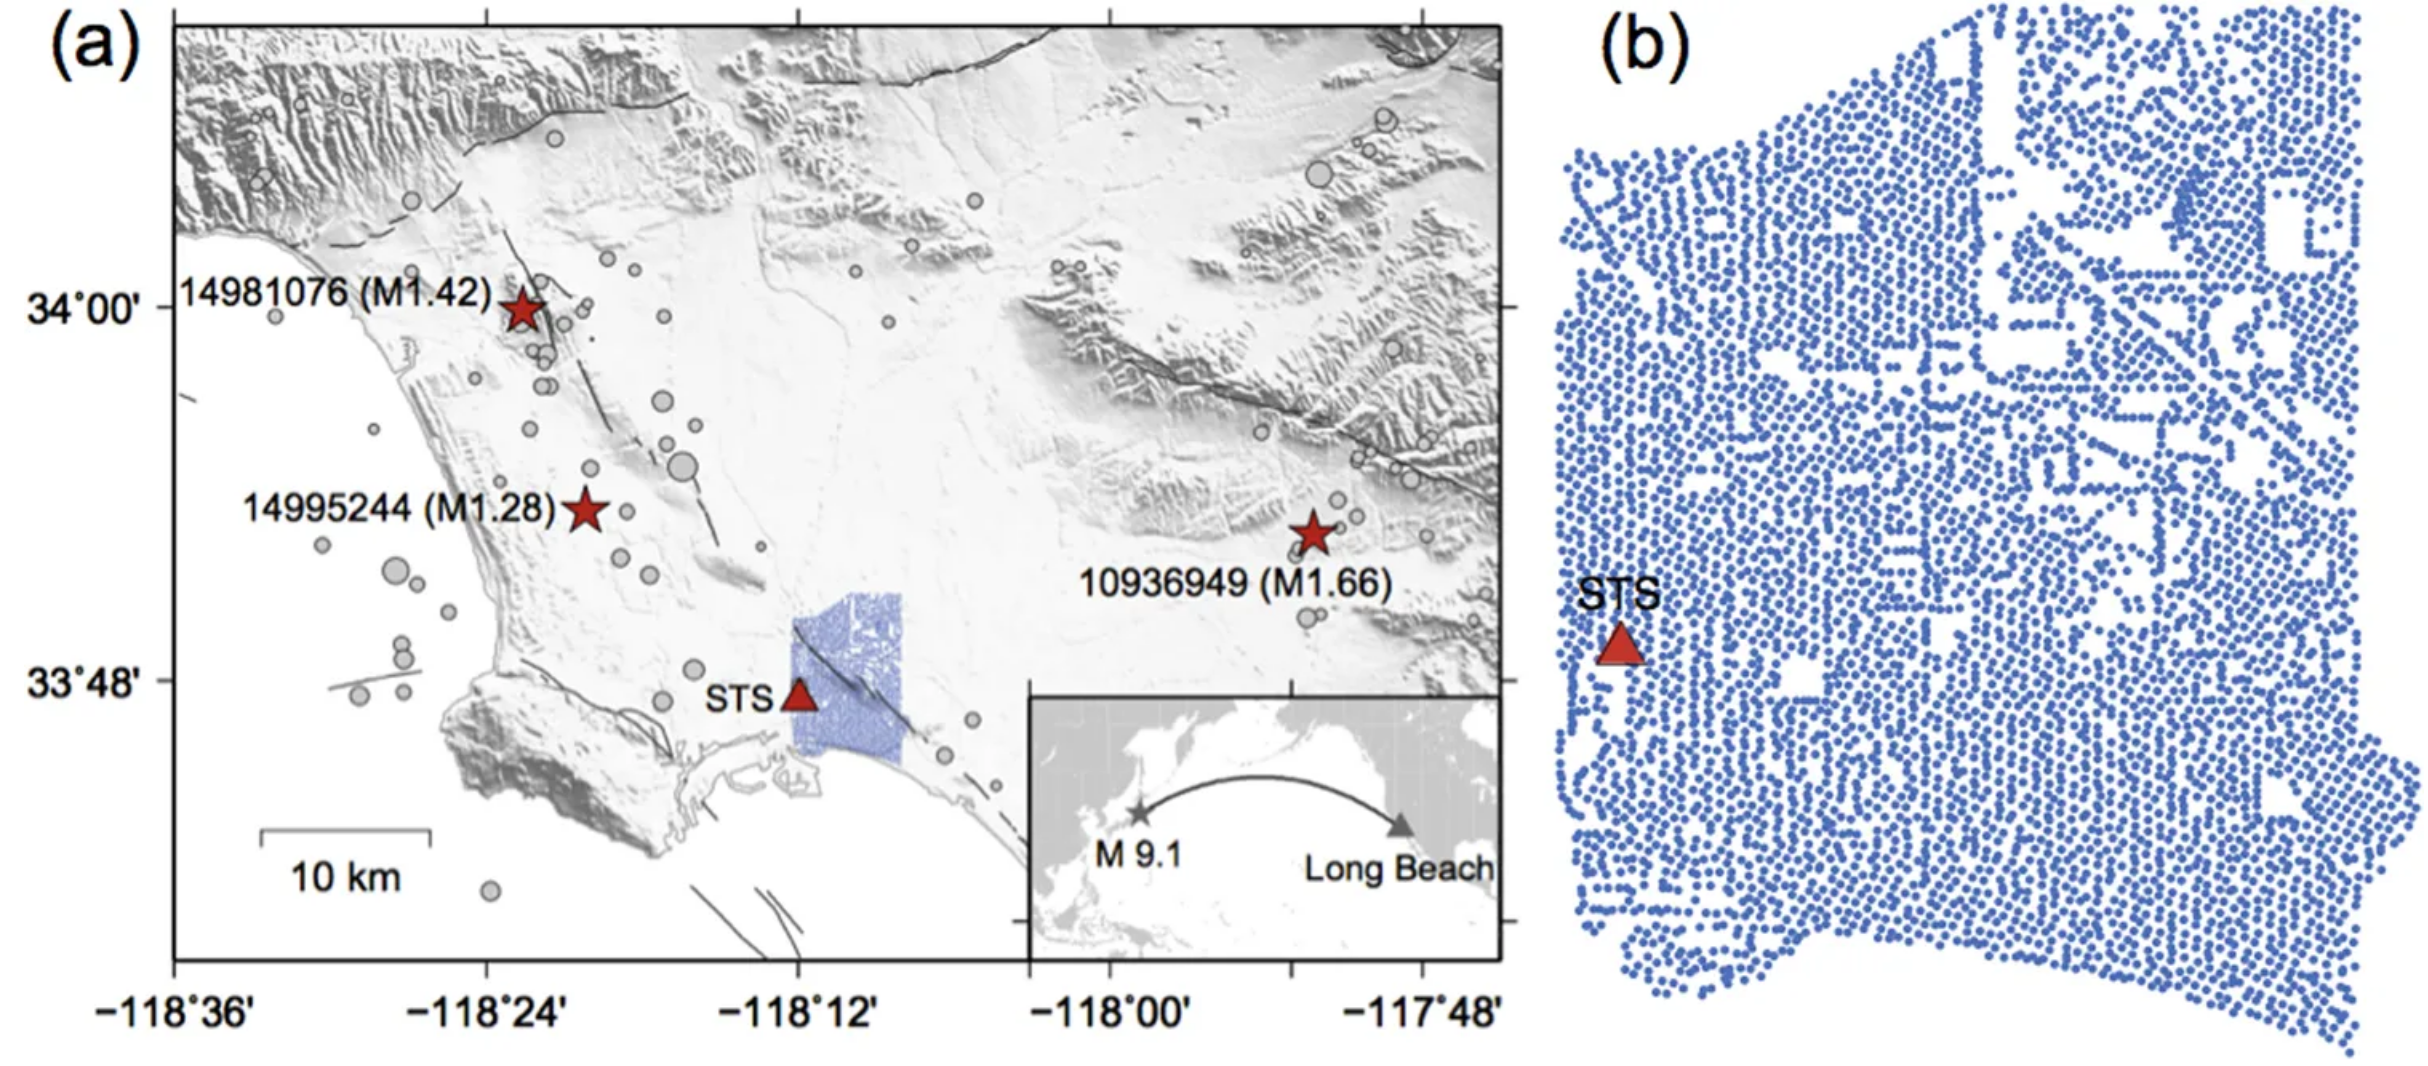
\includegraphics[width=\linewidth]{nodal_array}
    \caption{(a) Map of study region in \textcite{li2018high} for the Long Beach nodal array and local seismicity. (a) Blue dots are the 5200-sensor nodal array. A red triangle marks the broadband station STS belonging to Southern California Seismic Network (SCSN). Black curves denote the surface trace of mapped faults. Gray solid circles are seismicity listed in the SCSN catalog between January and June 2011, whose sizes are proportional to the magnitude. Red stars mark three selected cataloged events used for tests. The inset map shows locations of the $M_w$\,9.1 Tohoku-Oki earthquake and its ray path to Long Beach. (b)~Zoomed-in plot of the Long Beach array and the STS station. }
    \label{fig:nodal_array}
\end{figure}
%
While nodal array systems enable the deployment of dense sensor arrays at lower costs than ever before, their recording time is limited to relatively short time periods (weeks to months) on a stand-alone battery.

Systems monitoring seismic activity over mobile devices, such as a smartphone, were developed for \gls{eew} purpose \autocite{kong2016myshake}.
These low-cost, ``personal seismometers'' provide opportunities for long-term installations for wider coverage, especially in cities where it is difficult to deploy seismic sensors traditionally.
These systems build on the availability of inexpensive low-power embedded processors with commercial-grade accelerometers as their seismic sensors.
Accelerometers are ubiquitous in modern electronics, such as activating car airbags, rotating smartphone screens, and controlling gaming systems.
Even though the sensors in these devices are of lower quality compared to scientific-grade instruments, they are adequate to capture moderate to strong ground motions and are readily available for broader coverage of large monitoring regions.
Similar sensors have been installed in buildings to study the structural sway when a passing earthquake wave \autocite{kurata2017development}.

%
\begin{figure}
    \centering
    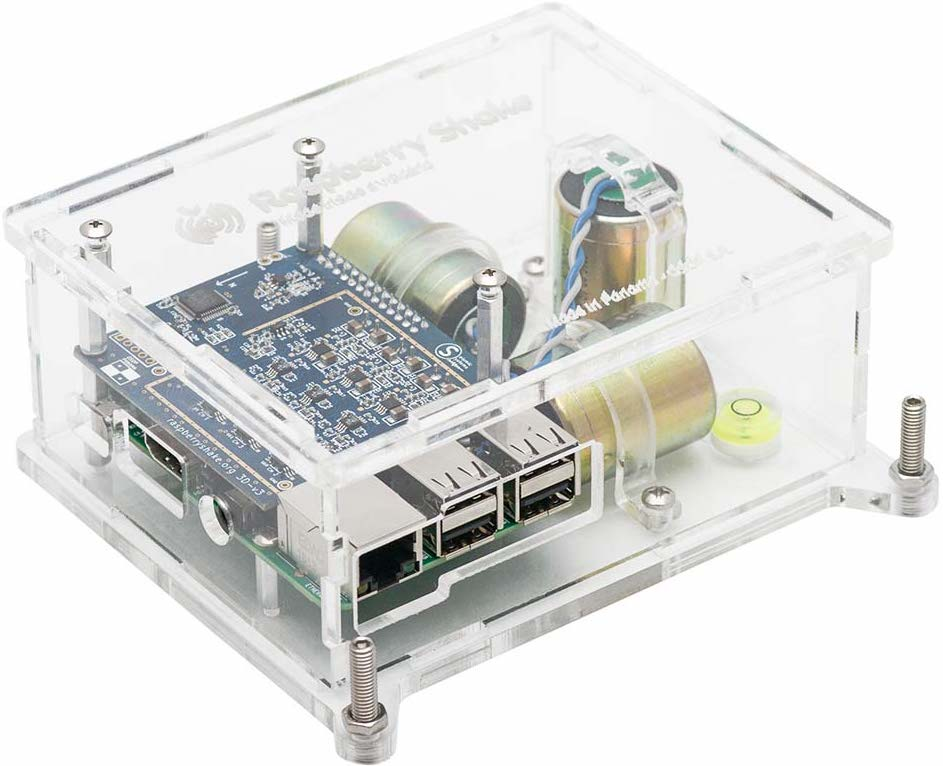
\includegraphics[width=0.8\linewidth]{raspberry_shake}
    \caption{Raspberry Shake 3D consisting of Raspberry Pi computer plus three vertical geophones with 100\,Hz sampling rate.}
    \label{fig:raspberry_shake}
\end{figure}
%
In the wake of embedded processing requirements of real-time seismic sensors, the Raspberry Shake (Figure~\ref{fig:raspberry_shake}) devices were developed with a large variety of configurations containing typical seismic sensors.
The onboard Raspberry Pi processor, which provides a four-core 1.4\,GHz CPU and 1\,GB of on-chip RAM, is a widely used embedded processing platform with extendibility potential to different types of sensor and communication modules \autocite{upton2014raspberry}.
Raspberry Shake sensors have been added to existing local seismic networks to complement the observations for moderate to large earthquakes, including in countries with more limited seismic monitoring infrastructure \autocite{christensen2017raspberry}.
\textcite{anthony2018low} confirmed the effectiveness of the Raspberry Shake system on both field and laboratory observations.
Different studies are being conducted to validate applications of the Raspberry Shake in many scenarios, including rockfall activity monitoring \autocite{manconi2018evaluation}, as well as local \autocite{christensen2017raspberry}, regional \autocite{pulli2018seismic}, and national seismic monitoring \autocite{calais2019can}.
The Raspberry Shake has proven to be not only a good development platform but also a viable deployment system for real-time acquisition and processing of seismic waveforms.
However, due to the limited computing resource on most of the embedded processors, a pre-trained full \gls{nn} model from a workstation cannot be directly deployed without further simplification.

\section{Computation on Hardware}
\label{sec:hardware}
%

\subsection{Convolution Strategies}
\label{sec:conv}
%
The basis of a \gls{cnn} model is the convolution operator between the input feature maps and the filter weights.
Three different strategies have been proposed to implement a convolution operator, namely direct convolution, unrolling based convolution, and \gls{fft} based convolution.
The direct convolution computes the convolution via a sliding window of filter weights over the feature maps which computes their dot product.
With proper padding and striding, the output can be formed into the desired shape.
This approach is adopted by cuda-convnet2 \autocite{krizhevsky2014one}, and Theano-legacy \autocite{bergstra2010theano,bastien2012theano}.
However, this direct approach usually results in a rather implementation.
\textcite{chetlur2014cudnn} used a memory heavy, but more efficient way to compute the convolution operator.
Each sliding window is unrolled into a row of a larger feature map matrix and the corresponding filter kernel is unrolled into a column of filter matrix.
The convolution operation is then reduced to multiplying the filter matrix by the feature map matrix.
Obviously, there are redundant entries in both matrices meaning that it uses more memory to store the intermediate values than the direct approach.
On the other hand, the convolution operation involves moving a considerable amount of data in and out the processor which is usually the bottleneck instead of the actual computation.
Converting the convolution to matrix multiplication gives a faster run time, because it performs a higher ratio of operations per byte of data transferred.
This ratio increases as the matrices get larger, so we want to form the largest matrix multiplication that the memory supports.
This unrolling based convolution approach is also adopted by many popular Frameworks including Caffe \autocite{jia2014caffe}, Torch \autocite{collobert2011torch7}, Theano \autocite{bastien2012theano} and later inherited by TensorFlow \autocite{abadi2016tensorflow} and PyTorch \autocite{paszke2017automatic}.
\textcite{vasilache2014fast} proposed the \gls{fft} based scheme that converts the time-domain convolution into a product in the Fourier domain.
This conversion significantly reduces the computational complexity; however, the overhead of converting between the time domain and Fourier domain makes it less efficient for smaller filters.
A detailed comparison of these three strategies is given by \textcite{li2016performance}.
Since the filter size in the \gls{cpic} model is either 3 or 5, the unrolling approach is preferred in this work.

\subsection{Matrix-matrix multiplication}
\label{sec:mmm}
%
%
The computation for \glspl{fc} can be easily represented as a matrix-matrix multiplication operation.
Since we adopt the unrolling approach in Section~\ref{sec:conv}, the convolution operations for the \glspl{conv}, which can be represented as a series of convolutional matrices, also consists of many matrix-matrix multiplications.

Indeed, consider a one layer in a CNN of the \gls{cpic} model as an example.
There are $M$ channels of inputs $x_m[n]$ for $m=1,2,\ldots, M$, each of length $N$, i.e., $n=0,1,\ldots N-1$.
The \gls{conv} produces $K$ channels of outputs $y_k[n]$ for $k=1,2,\ldots, K$, also of length $N$ (prior to max pooling).
Each input is connected to all outputs via 1-D convolution, where the filter length is $L$ and the filter coefficients (called the impulse response in DSP) are $h_{k,m}[n]$ for $n=0,1,\ldots, L-1$.
Thus we have $MK$ filters\,--\,all with different filter coefficients.
Altogether, there are $MLK$ parameters needed to define all the filters.
The $k$-th output channel, which is the sum of $M$ filtered inputs, becomes
\begin{equation}
y_k[n] = \sum\limits_{m=1}^{M} h_{k,m} \ast x_m
 = \sum\limits_{m=1}^{M} \sum\limits_{\ell=0}^{L-1} h_{k,m}[\ell]\, x_m[n-\ell]
\qquad\text{for\ } n=0,1,\ldots,N-1
\label{eq:conv_gemm}
\end{equation}
where $\ast$ denotes 1-D convolution.

One-dimensional convolution for one output channel can be expressed as a matrix-vector multiplication.
Since the length of the filters is much less than the input signal lengths, it is best to create the convolution matrices from the $M$ input channels.
The result is an $(N+L-1\times L)$ matrix $\bm X^{\text{Full}}_m$, where each column of $\bm X^{\text{Full}}_m$ contains all the signal values in the $m$-th input channel.
Successive columns are staggered by the stride length.
When the stride is one, the result is a Toeplitz matrix.
%If we define the $m$-th signal vector as $\bm x_m = [x_m[0]\; x_m[1]\, \ldots \, x_m[N-1]]^T$, then
Here is an example for $N=7$ and $L=3$ (the subscript $m$ is dropped from $x_m$), where the matrix is $(N+L-1)\times L = 9\times 3$:
\begin{equation*}
 \bm X^{\text{Full}}_m =
\begin{bmatrix}
x[0] & 0    & 0\cr
x[1] & x[0] & 0 \cr
x[2] & x[1] & x[0] \cr
x[3] & x[2] & x[1] \cr
x[4] & x[3] & x[2] \cr
x[5] & x[4] & x[3] \cr
x[6] & x[5] & x[4] \cr
0    & x[6] & x[5] \cr
0    & 0    & x[6] \cr
\end{bmatrix}
\qquad \text{Full Convolution matrix is } 9\times 3
\end{equation*}
If we want the output channels to have the same length as the input channels, we must remove two rows\,---\,conventionally the first and last, or the last two, and then we call the resulting matrix $\bm X_m$.
To get the matrix-vector form of convolution, we now define a length-$N$ column vector for the $k^\text{th}$ channel of output, $y_k[n]$, as
\[
 \bm y_k = 
 \begin{bmatrix} y_k[0] & y_k[1] & \ldots & y_k[N-1] \end{bmatrix}^T
\]
and a length-$L$ column vector for a filter between $m^\text{th}$ input channel and $k^\text{th}$ output channel
\[
 \bm h_{k,m} = 
 \begin{bmatrix} h_{k,m}[0] &  h_{k,m}[1] & \ldots & h_{k,m}[L-1] \end{bmatrix}^T
\]
The matrix-vector form for the convolution in \eqref{eq:conv_gemm} becomes
\[
\bm y_k = \sum\limits_{m=1}^{M} \bm X_m \bm h_{k,m}
=
\begin{bmatrix}
\bm X_1^{\phantom{.}} &  \bm X_2^{\phantom{.}} & \ldots & \bm X_M^{\phantom{.}}
\end{bmatrix}
\underbrace{\begin{bmatrix}
\bm h_{k,1} \cr  \bm h_{k,2} \cr  \vdots \cr  \bm h_{k,M}
\end{bmatrix}}_{\text{kernel}}
\]
Now we put all convolution matrices into one matrix $\bm X = \begin{bmatrix}
\bm X_1^{\phantom{.}} &  \bm X_2^{\phantom{.}} & \ldots & \bm X_M^{\phantom{.}}
\end{bmatrix}
$
and define the \emph{kernel} for the $k^\text{th}$ output as a collection of filters,
$
\bm h_k =
\begin{bmatrix}
\bm h_{k,1}^T & \bm h_{k,2}^T &  \ldots &  \bm h_{k,M}^T
\end{bmatrix}^T
$.
Finally, we write one matrix product for all the outputs of this single \gls{conv} as
\begin{equation}
\bm Y =
\begin{bmatrix}
\bm y_1^{\phantom{.}} & \bm y_2^{\phantom{.}} & \cdots & \bm y_K^{\phantom{.}}
\end{bmatrix}
= \bm X
\begin{bmatrix}
\bm h_{1}^{\phantom{.}} & \bm h_{2}^{\phantom{.}} & \cdots & \bm h_{K}^{\phantom{.}}
\end{bmatrix}
= \bm X \bm H
\label{eq:conv_gemm_mtx}
\end{equation}
where $\bm Y$ is $N\times K$, $\bm X$ is $N\times ML$, and $\bm H$ is $LM\times K$.

Figure~\ref{fig:gemm} gives an example of such an unrolled convolution between a $3 \times 6$ input feature map ($X_{ij}$) and two three-channel convolution kernels ($H_{ij}$ and $G_{ij}$).
Convolution matrices of the feature map with full zero-padding are constructed for each input channel (represented in three different colors) and concatenated horizontally into one \textbf{input matrix}. 
Since the stride value in this example is $1$, notice that the matrix structure inside each colored block of the \textbf{input matri}x is Toeplitz.
If a stride value larger than $1$ is used, some of input matrix rows are removed for the corresponding windows skipped due to the larger stride value.
On the right hand side, the filter weights of different input channels are concatenated vertically  into columns of the \textbf{kernel matrix} according to the channel order in the input matrix (using the same color code).
Different filters are stacked horizontally to so that their outputs can be computed simultaneously.
Note that the kernel matrix is invariant to the specific stride choice.
Thus, the computation of the output (yellow) for this \gls{conv} can be represented as a multiplication between the input and kernel matrices.
%
\begin{figure}
    \centering
    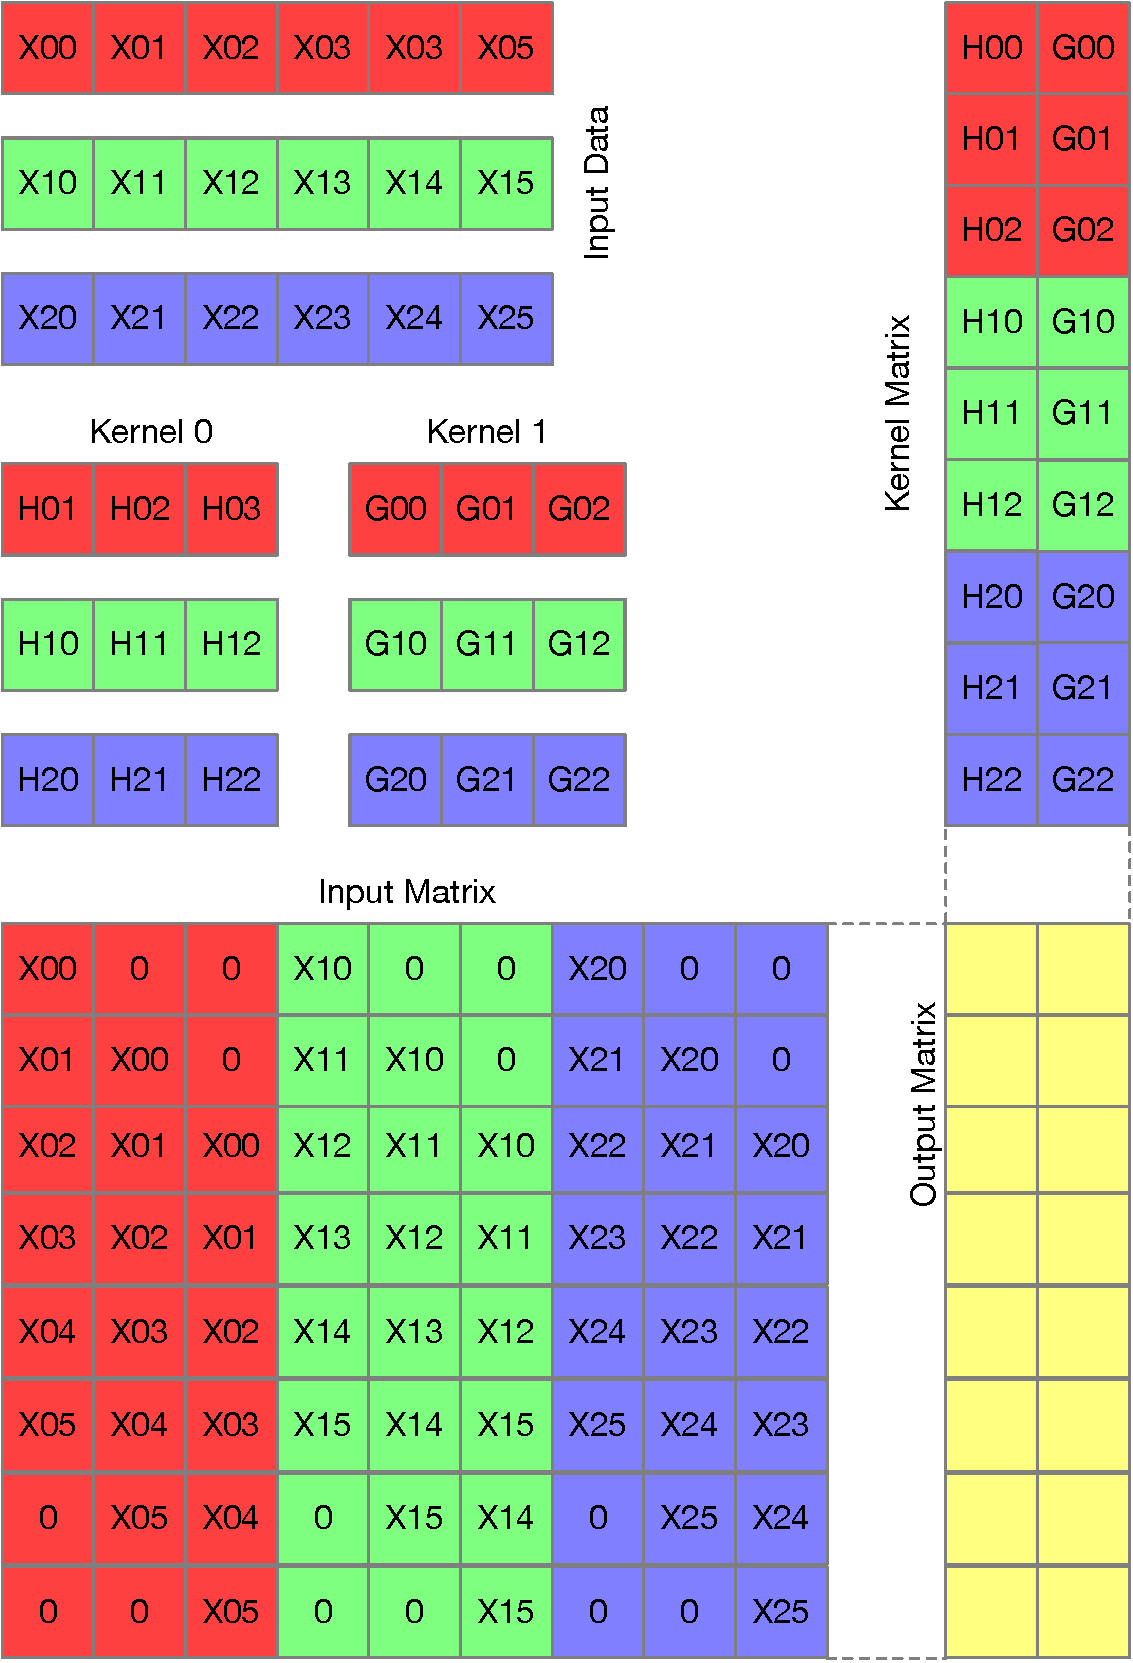
\includegraphics[width=0.9\columnwidth]{gemm}
    \caption{Convolution example (with zero-padding) between a three input channels and two size-9 kernels. Notice that $M=3$, $N=6$, $L=3$, and $K=2$ as defined in \eqref{eq:conv_gemm}.}
    \label{fig:gemm}
\end{figure}
%

As a result, accelerating the computation of matrix-matrix multiplication (e.g., $\bm C = \bm A \bm B$) can significantly improve the computation of the overall \gls{cpic} model, which relies on \glspl{conv} and one \gls{fc}.
Such operations are conventionally performed by a function called \gls{gemm}.
Most \gls{gemm} functions from the \gls{blas} are optimized for scientific computing where matrices might be as large as thousands of double-precision floating-point elements.
Thus, these \gls{gemm} functions typically repack two matrices $\bm A$ and  $\bm B$ into smaller shapes as shown in Figure~\ref{fig:hardware_implmentation} when the overall matrix size exceeds the L1 cache size of the microkernels.
Each pair of these smaller matrices is fed into a microkernel to compute their product and accumulated outside for the final results.
The bottom line is using fewer filters in each kernel, or fewer kernels, can significantly reduce the overall computation cost.

Another issue is number representation.
When fixed-point numbers are used for the seismic acquisition system, it is natural to use fixed-point numbers for the CNN computation as well. 
However, when using the same \gls{gemm} functions, accumulation of fixed-point numbers outside the microkernel might be necessary but is very undesirable.
Instead, using lower-precision fixed-point numbers is preferred so that the entire dot product can be computed at once inside a single microkernel at high precision as shown in Figure~\ref{fig:hardware_implmentation}.
Then the dot product result is shifted back into a compatible lower-precision fixed-point number as the output of the microkernel.
This puts an additional constraint on the system design that the memory required for each dot product block needs to be less than the L1 cache size of the processor.
Note that most embedded processors, including the Raspberry Pi, have more than 16\,KB of L1 cache.
This allows multiple outputs to be computed inside each microkernel as shown in Figure~\ref{fig:hardware_implmentation} using lower-precision numbers, which further improves the computation efficiency.
%
\begin{figure}
    \centering
    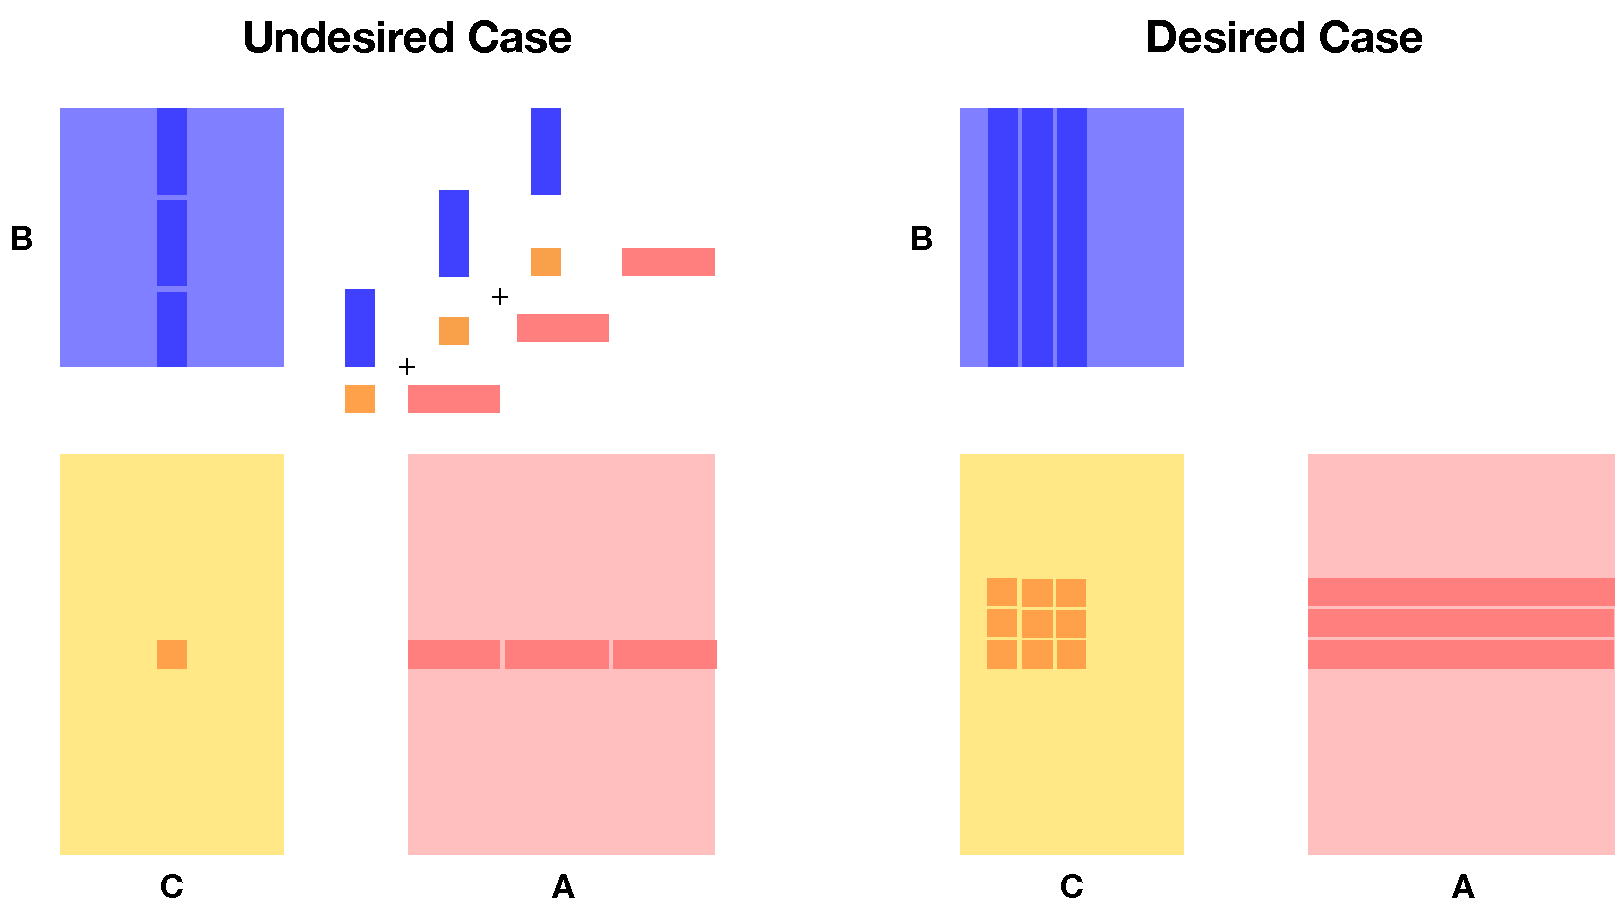
\includegraphics[width=\linewidth]{hardware_implementation}
    \caption{\gls{gemm} implementations for (undesired case, left) high-precision floating-point system where rows and columns must be broken up to compute one output of the large matrix, and (desired case, right) low-precision fixed-point system where entire rows and columns are available in the L1 cache to create small submatrices of the output.}
    \label{fig:hardware_implmentation}
\end{figure}
%


\section{Visualizing CNN filter weights}
\label{sec:visualization}
%
To simplify the \gls{cpic} model, two approaches are studied in this section.
First, by visualizing the filter weights, redundant filters can be identified and removed. After such pruning the entire \gls{cnn} model must be fine-tuned and revalidated to make sure that the desired classification accuracy is maintained on the simplified model.
Second, the distribution of filter weights on each \gls{conv} spans a relatively consistent dynamic range.
This property allows us to use a lower-precision fixed-point number representation,
because the small errors in number representation should not change the classification outputs very much.
Both of these phenomena can be exploited to further simplify the \gls{cnn} model complexity, as well as reduce the memory cost.

\subsection{CNN Filter Weights Close to Zero}
\label{sec:zero_weights}
%
Although there are many filters within each layer of the original \gls{cpic} model, there exist some filters most of whose weights are very close to zero.
These filters can be found by visualizing the magnitude of each kernel's filter weights as a 2-D image.
Eliminating such kernels helps to reduce unnecessary computation and memory usage while having little effect on the final classification results.
This process is known as network pruning.

%
\begin{figure}
    \centering
    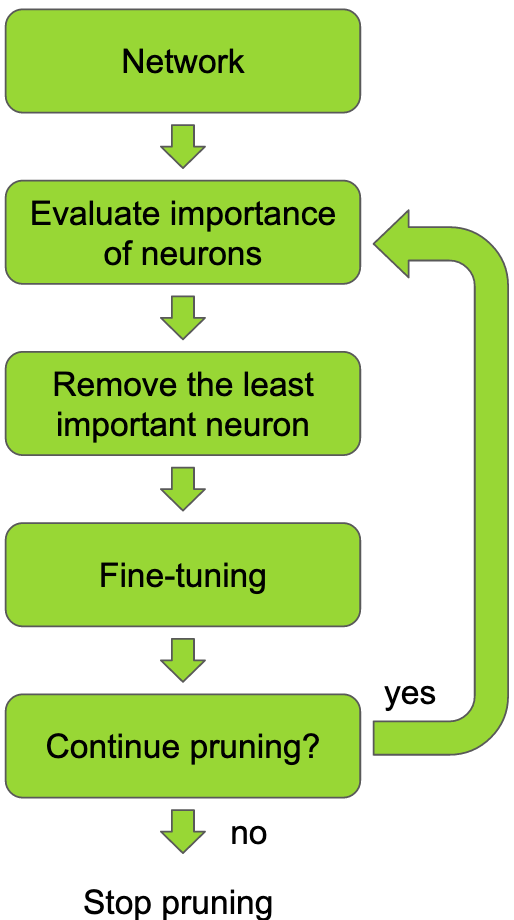
\includegraphics[width=0.32\linewidth]{pruning}
    \caption{Flow diagram of neural network pruning as a backward filter presented as Figure 1 in  \textcite{molchanov2016pruning}.}
    \label{fig:pruning}
\end{figure}
%
The general steps of network pruning \autocite{li2016pruning} are shown in Figure~\ref{fig:pruning}: the importance of each neuron is evaluated by looking at the effect of its filter weights.
A computationally costly scheme of ranking the importance of each neuron has been proposed by \textcite{molchanov2016pruning} from Nvidia; a similar approach was proposed by \textcite{anwar2017structured} as well.
These techniques prune the network by running the following optimization program:
%
\begin{equation}
\min_{\mathcal{W}'} \left|\mathcal{C} (\mathcal{D} | \mathcal{W}') - \mathcal{C} (\mathcal{D} | \mathcal{W})\right|, \text{ s.t. } \| \mathcal{W}' \|_0 \leq B
\label{eq:pruning}
\end{equation}
%
where $\mathcal{W}$ is the filter weights, $\mathcal{C}$ is the final classification accuracy, $\mathcal{D}$ is the training data, and $B$ is a positive integer.
Although \eqref{eq:pruning} is the ultimate goal one would want for network pruning, solving it requires exhaustively trying out all possible combinations of removing different redundant weights.
Such a solver requires a massive amount of computing power that is not commonly available except at those organizations with large computing clusters having thousands of \glspl{gpu}, such as Nvidia.
More importantly, the pruned network is optimized for a fixed set of data and fine-tuning of the pruned model would require repeated runs of the optimization program in \eqref{eq:pruning}.
This is not possible on any existing edge device, nor preferable, since the model on the edge needs to be self-adaptive to new incoming waveforms at a reasonable computing cost.

Instead of looking at individual filter weights, each filter and kernel must be treated as a whole and kept or removed altogether.
By visualizing filter weights and looking for kernels whose weights are mostly close to zero, the kernels with most of their weights close to zero are identified. 
By removing those kernels, the minimum number of kernels are determined for each layer.
The absolute value of the filter weights within \gls{cpic} layers are shown in  Figures~\ref{fig:cpic_weights_first_two}\,--\,\ref{fig:cpic_weights_fc}.
At the $i$-th layer, the $M_i$ filters connected to one output make up the kernel for that output.
Each kernel is displayed as a rectanguar image, and one row of the image is one of the filters within a kernel.
All kernels within the same layer are shown side by side in Figures~\ref{fig:cpic_weights_first_two}\,--\,\ref{fig:cpic_weights_fc}.
Note that filter weights are hard-clipped at 10 to highlight the difference between small and large filter weights.
Yellow and cyan regions correspond to weights with large magnitudes, while the black regions correspond to those with close to zero magnitudes.
Since there are only a limited number of kernels ($K_i$) in each layer, the number of kernels having all weights close to zero is easy to count.
%
\begin{table}
    \centering
    \caption{Number of kernels in each layer of the \gls{cpic} model during every iteration of the network pruning process.}
    \label{tab:pruning}
    \scalebox{0.93}{
        \begin{tabular}{l c c c c c c c c c c c c}
            \toprule
            Layer & 1 & 2 & 3 & 4 & 5 & 6 & 7 & 8 & 9 & 10 & 11 & fc\\
            \midrule
            Original number of kernels & 16 & 32 & 64 & 64 & 64 & 64 & 64 & 64 & 64 & 64 & 64 & 64\\
            \# close-to-zero kernels & 9 & 13 & 25 & 26 & 28 & 22 & 30 & 30 & 30 & 31 & 44 & 24\\
            1st iteration number of kernels & 8 & 16 & 32 & 32 & 32 & 32 & 32 & 32 & 32 & 32 & 16 & 32\\
            2nd iteration number of kernels & 8 & 16 & 32 & 32 & 32 & 16 & 16 & 16 & 16 & 16 &  \colorbox{red}{0} & 32\\
            3rd iteration number of kernels & 8 & 16 & 32 & 32 & 32 & 16 & 16 & 8 & 8 & 8 &  \colorbox{red}{0} & 32\\
            4th iteration number of kernels & 8 & 16 & 16 & 32 & 16 & 8 & 8 & 4 & 4 & \colorbox{red}{0} &  \colorbox{red}{0} & 16\\
            5th iteration number of kernels & 8 & 16 & 16 & 32 & 32 & 16 & 16 & 8 & 8 &  \colorbox{red}{0} &  \colorbox{red}{0} & 32\\
            \bottomrule
    \end{tabular}}
\end{table}
%
In Figure~\ref{fig:cpic_weights_first_two}, nine filters in layer \#1 and 13 filters in layer \#2 are close to zero.
This is a clear indication that the \gls{cpic} model can be simplified by removing those filters with small weights.

Unfortunately, the percentage of close-to-zero kernels is less on the deeper layers.
Figure~\ref{fig:cpic_weights_deep_layers} shows the weights on layer \#4, layer \#7, and layer \#11, respectively.
Even though there are still kernels on layers \#4 and \#7 whose weights are almost all close to zero, many of them tend to have a small number of large weights, with the rest close to zero.
On layer \#11, the situation becomes similar to the first two layers where a majority of the  kernels (56 out of 64) have all their weights close to zero.

In Figure~\ref{fig:cpic_weights_fc}, the weights on the \gls{fc} are shown with dynamic ranges clipped between 0 and 1.
With 64 inputs and 3 outputs, some of the weights on this \gls{fc} are clearly close to zero.
When a column of this image is all zero, that input feature doesn't matter for classification.
For Figure~\ref{fig:cpic_weights_fc}, this indicates that the final classifier made its decision on a small subset of the features in the total 64-element feature space.
Thus, it is likely that the \gls{cpic} model can be further simplified by using a smaller feature space for classification.
%
\begin{figure}[h!]
    \centering
    \begin{subfigure}{\linewidth}
        \centering
        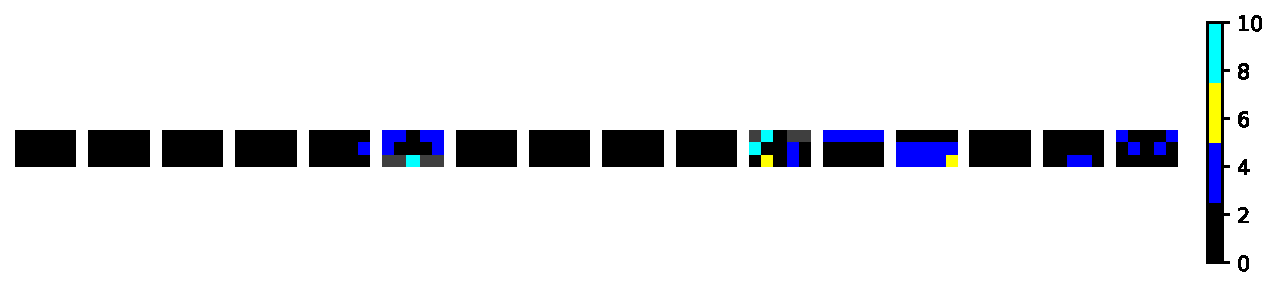
\includegraphics[width=\linewidth]{cpic_original_layer1}
        \caption{Layer \#1: 9 (out of 16) kernels close to zero at $k=1,2,3,4,7,8,9,10,14$ }
    \end{subfigure}
    %
    \begin{subfigure}{\linewidth}
        \centering
        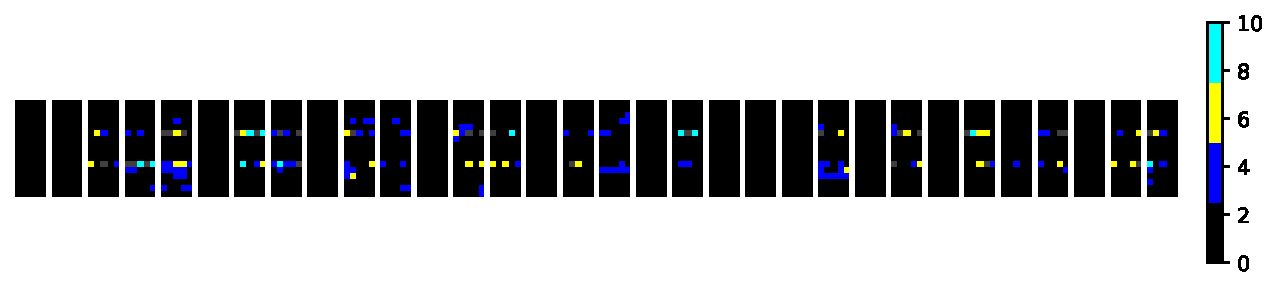
\includegraphics[width=\linewidth]{cpic_original_layer2}
        \caption{Layer \#2: 13 (out of 32) kernels close to zero\\ \rule{59mm}{0pt} at $k=1,2,5,8,11, 14,17,19,20,21, 23,25,26,30$}
    \end{subfigure}
    %
    \caption{Absolute values of the filter weights in the first two layers of the \glstext{cpic} model which use 5-point convolutions. For each subimage one row is a filter, so the horizontal dimension is $L_i=5$, and the vertical dimension is $M_i$, the number of layer inputs, 3 for layer \#1 and 16 for layer \#2. The number of subimages is equal to the number of layer outputs, $K_1=16$ for layer \#1 and $K_2=32$ for layer \#2.  See Figure~\ref{fig:cnn} in Chapter 2 for a diagram of the entire \gls{cnn}.}
    \label{fig:cpic_weights_first_two}
\end{figure}
%
\begin{figure}
    \centering
    \begin{subfigure}{\linewidth}
        \centering
        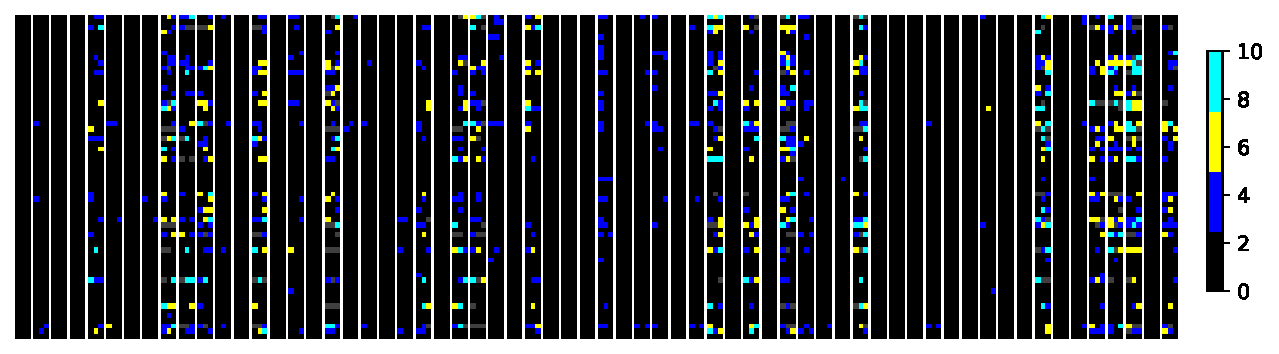
\includegraphics[width=\linewidth]{cpic_original_layer4}
        \caption{Layer \#4: 26 (out of 64) kernels close to zero\\ \rule{0mm}{0pt}
        	 for $k=1, 3, 4, 7, 13, 15, 17, 21, 24, 28, 30, 31, 32, 34, 37, 40, 42, 48, 49, 50, 52, 53, 55, 56, 58, 63$}
    \end{subfigure}
    %
    \begin{subfigure}{\linewidth}
        \centering
        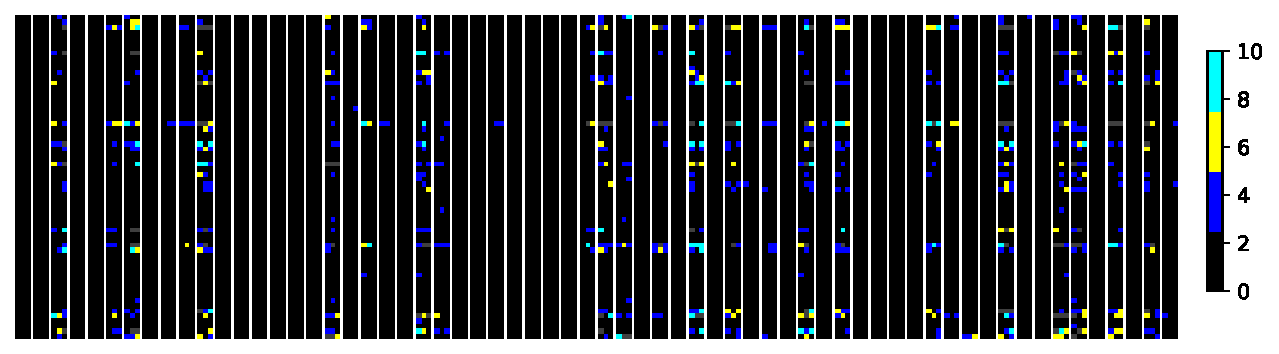
\includegraphics[width=\linewidth]{cpic_original_layer7}
        \caption{Layer \#7: 30 (out of 64) kernels close to zero\\ \rule{10mm}{0pt}
         for $k=1, 2, 4, 5, 8, 12, 13, 14, 15, 16, 17, 22, 25, 26, 28, 29,$
         \\ \rule{55mm}{0pt}$ 30, 31, 35, 37, 39, 43, 47, 48, 49, 50, 54, 57, 60, 62$}
    \end{subfigure}
    %
    \begin{subfigure}{\linewidth}
        \centering
        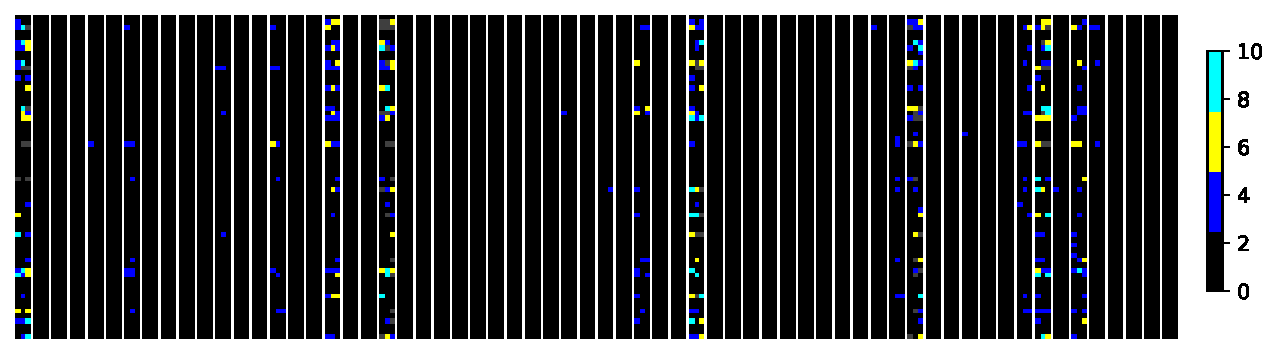
\includegraphics[width=\linewidth]{cpic_original_layer11}
        \caption{Layer \#11: 44 (out of 64) kernels close to zero;\\ \rule{10mm}{0pt}
        	 nonzero for $k=1, 5, 7, 12, 15, 18, 21, 31, 33, 35, 38, 48, 49, 50, 53, 56, 57, 58, 59, 60$}
    \end{subfigure}
    %
    \caption{Absolute value of the filter weights in \glstext{conv}s with length-3 filters where $L_i=3,\ M_i=64,\ K_i=64$: (a) layer \#4 (b) layer \#7; and (c) layer \#11. At least half of the kernels in most layers are close to zero. The number of kernels close to zero (black) increases, and then decreases, in the deeper layers. }
    \label{fig:cpic_weights_deep_layers}
\end{figure}
%
%
\begin{figure}
    \centering
    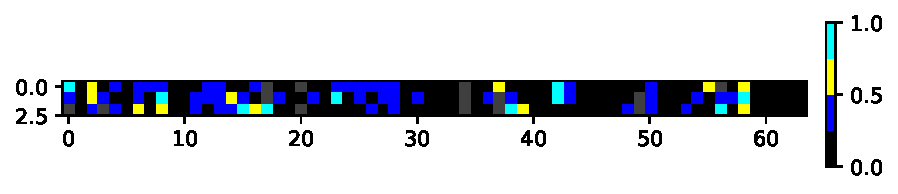
\includegraphics[width=\linewidth]{cpic_original_fc}
    \caption{Filter weights in the \glstext{fc} of \glstext{cpic} model with 64 inputs and 3 outputs. Each column represents the three weights from one input neuron to all three output neurons. Approximately 30 of these columns have all weights close to zero. Note that the dynamic range of these images is reduced to lie between $0$ and $2$.}
    \label{fig:cpic_weights_fc}
\end{figure}
%

This pruning process can be conducted multiple times to further reduce the overall number of kernels (and individual filters).
Empirically, the pruned model achieves better classification results by fine-tuning on a series of models whose kernels are gradually removed instead of a single model with all redundant kernels removed at once.
Table~\ref{tab:pruning} records the number of kernels on each layer during five pruning iterations. 
During the second and fourth iterations, the number of kernels on the last \gls{conv} is small enough that we merge it with the previous layer.
This reduces the overall number of layers.
After the fourth pruning iteration, the resulting model experienced a severe drop in the classification accuracy.
We suspect that the model complexity was reduced too much, and the simplified model was unable to handle the variance inside the training dataset.
Thus, we add back additional kernels in the fifth iteration to increase the model complexity and ultimately decided to use nine \glspl{conv} in the final model.

\subsection{Distribution of the CNN Filter Weights}
\label{sec:weight_distribution}
%
In addition to the absolute value of the filter weights, the distribution of these weights on each layer must also be considered.
Distributions of the weight in all 11 \glspl{conv}, as well as the final \gls{fc} are shown in Figure~\ref{fig:weight_distribution} with 20 bins and a constant range from $-10$ to $+10$.
Except for the first \gls{conv}, the weight distributions on all the rest of the layers resemble each other.
More importantly, for all the layers these distributions are symmetric and tightly centered around zero.
This phenomenon allows us to use a fixed-point number system to represent the weights in lower precision and further reduces the memory, as well as the computation cost of the \gls{cpic} model.
Furthermore, a symmetric dynamic range of the fixed-point number can be adopted without a bias term due to the symmetry around zero in all the filter weight distributions.
On the other hand, there is no need to consider the bias term for the feature map distribution.
Since each \gls{conv} is followed by a \gls{relu} activation function, the resulting feature maps are also nonnegative which allows us to use unsigned fixed-point numbers to represent the feature map values.
%
\begin{figure}
    \centering
    %
    \begin{subfigure}{0.48\linewidth}
        \centering
        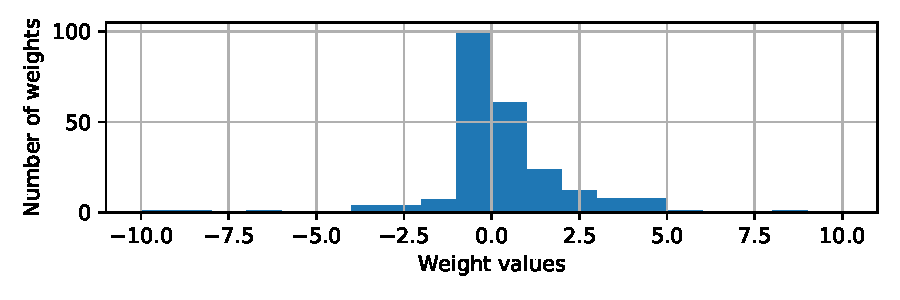
\includegraphics[width=\linewidth]{hist_layer1}
        \caption{\glstext{conv} \#1}
    \end{subfigure}
    \hfill
    \begin{subfigure}{0.48\linewidth}
        \centering
        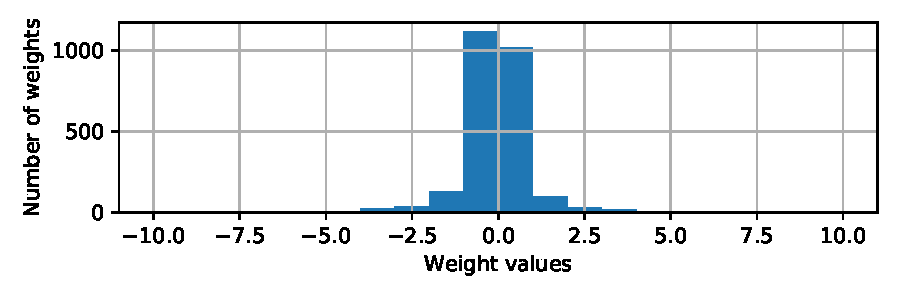
\includegraphics[width=\linewidth]{hist_layer2}
        \caption{\glstext{conv} \#2}
    \end{subfigure}
    %
    %
    \begin{subfigure}{0.48\linewidth}
        \centering
        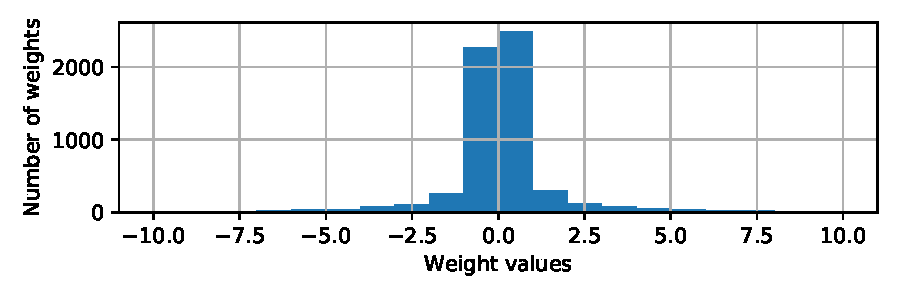
\includegraphics[width=\linewidth]{hist_layer3}
        \caption{\glstext{conv} \#3}
    \end{subfigure}
    \hfill
    \begin{subfigure}{0.48\linewidth}
        \centering
        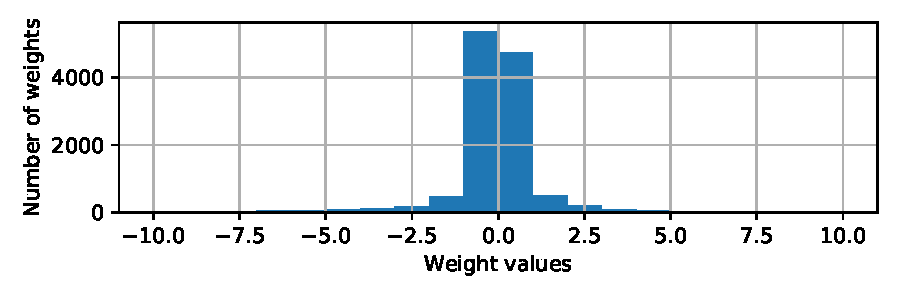
\includegraphics[width=\linewidth]{hist_layer4}
        \caption{\glstext{conv} \#4}
    \end{subfigure}
    %
    %
    \begin{subfigure}{0.48\linewidth}
        \centering
        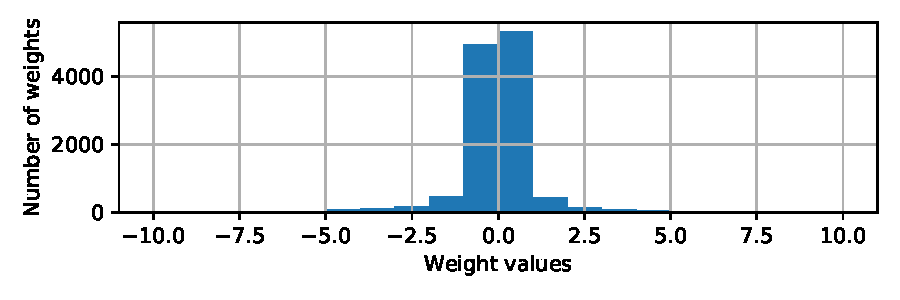
\includegraphics[width=\linewidth]{hist_layer5}
        \caption{\glstext{conv} \#5}
    \end{subfigure}
    \hfill
    \begin{subfigure}{0.48\linewidth}
        \centering
        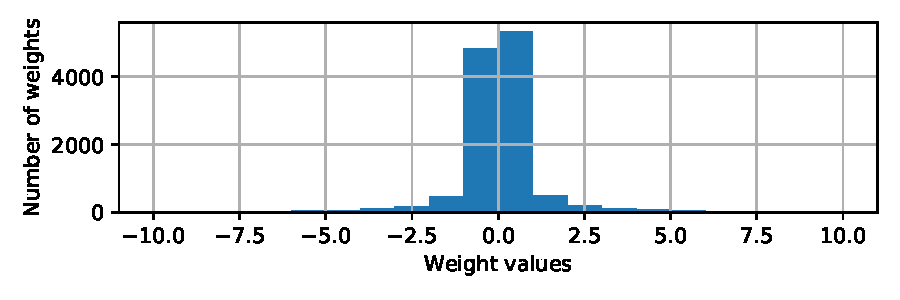
\includegraphics[width=\linewidth]{hist_layer6}
        \caption{\glstext{conv} \#6}
    \end{subfigure}
    %
    %
    \begin{subfigure}{0.48\linewidth}
        \centering
        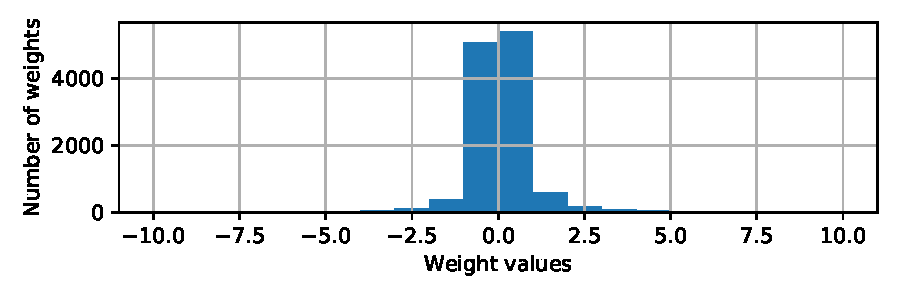
\includegraphics[width=\linewidth]{hist_layer7}
        \caption{\glstext{conv} \#7}
    \end{subfigure}
    \hfill
    \begin{subfigure}{0.48\linewidth}
        \centering
        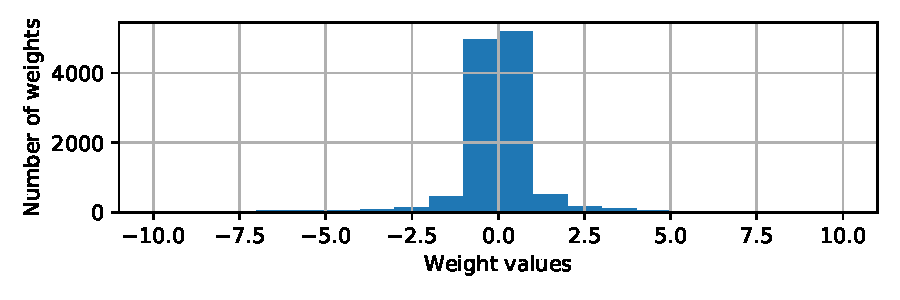
\includegraphics[width=\linewidth]{hist_layer8}
        \caption{\glstext{conv} \#8}
    \end{subfigure}
    %
    %
    \begin{subfigure}{0.48\linewidth}
        \centering
        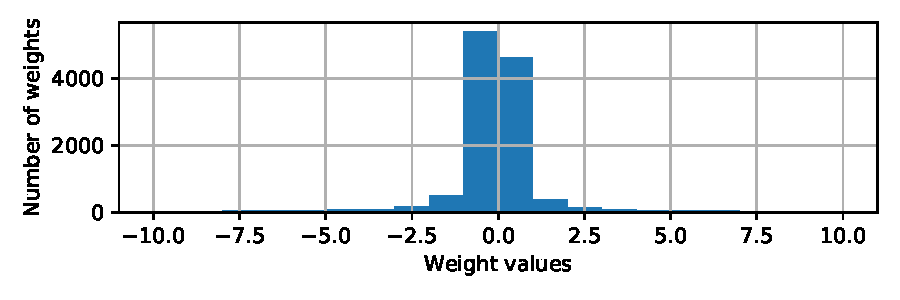
\includegraphics[width=\linewidth]{hist_layer9}
        \caption{\glstext{conv} \#9}
    \end{subfigure}
    \hfill
    \begin{subfigure}{0.48\linewidth}
        \centering
        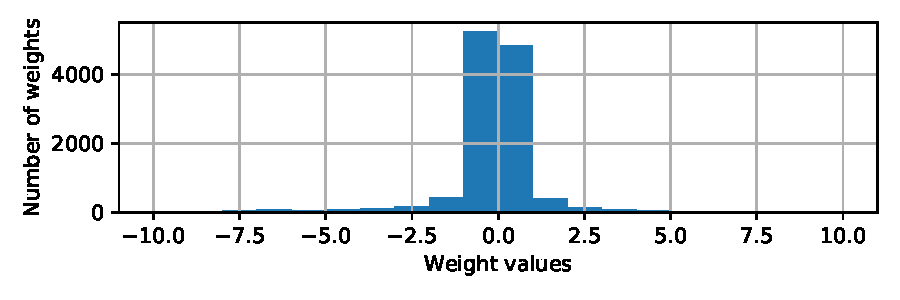
\includegraphics[width=\linewidth]{hist_layer10}
        \caption{\glstext{conv} \#10}
    \end{subfigure}
    %
    %
    \begin{subfigure}{0.48\linewidth}
        \centering
        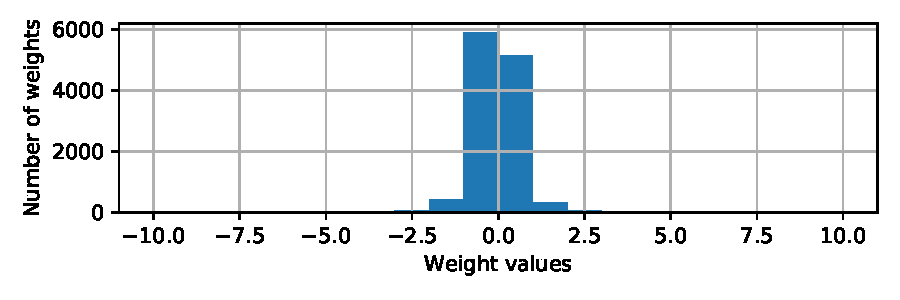
\includegraphics[width=\linewidth]{hist_layer11}
        \caption{\glstext{conv} \#11}
    \end{subfigure}
    \hfill
    \begin{subfigure}{0.48\linewidth}
        \centering
        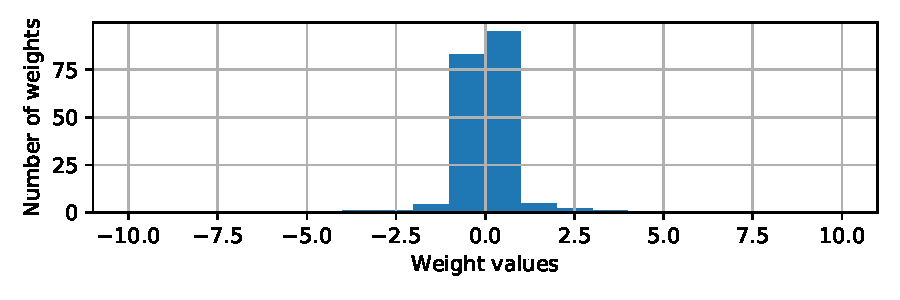
\includegraphics[width=\linewidth]{hist_fc}
        \caption{\glstext{fc}}
    \end{subfigure}
    %
    \caption{Distribution of filter weights on every layer of the \glstext{cpic} model before pruning. The total number of weights is $L_i M_i K_i$ for the $i$-th layer. Consult Table~\ref{tab:cnn_original} for the specific values of $L_i$, $M_i$ and $K_i$.}
    \label{fig:weight_distribution}
\end{figure}

\section{Model Simplification}
\label{sec:simplification}
% Model simplification need for deployment on raspberry pi
%   1. merge batch norm (n)
%   2. pruning features (n)
%   3. weight sharing (n)
%   4. quantization (y)
%   5. encoding (huffman encoding) (n)
%   6. hardware acceleration (TensorRT, QNNPACK) (n)

\subsection{Reducing Network Depth}
\label{sec:network_depth}
%
Since each \gls{conv} is followed by a max-pooling layer of size two, the size of the feature map in the time dimension is reduced by two following each \gls{conv}.
Thus, the overall downsampling ratio is controlled by the number of \glspl{conv}.
In order to reduce the model complexity by removing some of the \glspl{conv}, the duration of the input window could be shortened to have fewer time samples in the 3-C waveforms.
For different window lengths $T_w$, the labeled phase arrival time must always be positioned at $0.25T_w$ from the beginning.
As shown in Table~\ref{tab:window-length}, some other possible window lengths were tested, even a longer window, but a 20-s window duration works best for the Wenchuan dataset.
Recall that for each manually picked phase, \gls{cpic} uses a 20-s long window starting 5\,s before the pick and ending 15\,s after as one window of a seismic phase (Figure~\ref{fig:wenchuan_windows}).
Thus, removing layers by shortening the input window length is not a right approach.


Another approach is possible by examining the \gls{fc}.
Since the feature space sizes in the \glspl{conv} and the \gls{fc} have some redundancy as shown in Figures~\ref{fig:cpic_weights_deep_layers} and \ref{fig:cpic_weights_fc}, the trade-off between more \glspl{conv} vs.\ a larger \gls{fc} discussed in Section~\ref{sec:method-cnn} can be reconsidered.
In fact, the last few \glspl{conv} perform convolutions between a very short input signal and a small kernel which is nearly the same as a fully connected structure, so it is reasonable that these could be merged into the final \gls{fc}.
Specifically, we can gradually reduce the feature space size from 64 to 4 until the max-pooling layer reduces the number of time samples from 2,000 to 8.
This results in an $8\times 4$ feature tensor which can be flattened into a $32\times 1$ feature vector for the final \gls{fc}.
%
\begin{table}
    \centering
    \caption{Classifier accuracy (defined in \eqref{eq:accuracy}) vs.  window lengths.}
    \label{tab:window-length}
    \begin{tabular}{l c c c c c}
        \toprule
        Window Length (sec) & 2.5 & 5 & 10 & 20 & 40\\
        \midrule
        Accuracy(\%) & 94.7 & 96.3 & 96.9 & 97.4 & 97.2\\
        \bottomrule
    \end{tabular}
\end{table}
%



\subsection{Reducing Feature Space Size}
\label{sec:feature_size}
%
In Section~\ref{sec:visualization}, it is shown that all \glspl{conv} and the final \gls{fc} have some redundancy in the filter weights.
Thus, the overall number of filters on each layer, or the feature space size, can be reduced.
To present tweaking of an individual layer and demonstrate the overall effect on the model classification accuracy,  feature space sizes are reduced simultaneously with a fixed ratio on all layers.
Table~\ref{tab:feature_size} summarizes the \gls{cnn} model classification accuracy, given different levels of reduction in the feature space size on all layers.
The original \gls{cpic} model has a feature space size of 64 and reaches a classification accuracy of 97.4\%.
By reducing the feature space size to 32, the loss in classification accuracy is negligible (only 0.1\%).
However, further reduction in the feature space size to 16 results in a noticeable drop in the classification accuracy, although it is still within 1\% of the original model.
When the feature space size is reduced to 8, a drop of a little more than 1\% in classification accuracy is observed.
This serves as a guideline in simplifying the \gls{cnn} for improving the overall \gls{cpic} design.
%
\begin{table}
    \centering
    \caption{Classification accuracy (defined in \eqref{eq:accuracy}) vs. the final feature space size.}
    \label{tab:feature_size}
    \begin{tabular}{l c c c c}
        \toprule
        Feature Space Size & 8 & 16 & 32 & 64\\
        \midrule
        Number of parameters & 1972 & 7,320 & 30,544 & 107,248\\
        Accuracy (\%) & 96.3 & 96.8 & 97.3 & 97.4\\
        \bottomrule
    \end{tabular}
\end{table}

\subsection{Simplified Model}
\label{sec:simplified_model}
%
Combining the knowledge we gained from reducing model depth in Section~\ref{sec:network_depth} and reducing feature space size in Section~\ref{sec:feature_size}, we were able to further simplify the original \gls{cpic} model as shown in Figure~\ref{fig:cpicv2}.
The overall number of parameters decreases from 107,440 in the original \gls{cpic} model (Table~\ref{tab:cnn_original}) to 9,112 in the simplified model (Table~\ref{tab:cnn_simplified}), almost a factor of 12 reduction.
Following the observation in Section~\ref{sec:feature_size}, the most significant feature space size has been reduced from 64 to 32, which results in about a factor of three reduction in the number of parameters.
Based on the number of close-to-zero filters in the individual layers from Section~\ref{sec:visualization}, the numbers of filters on the deeper layers are no longer homogeneous.
Rather it decreases along with the time domain which results in a further reduction in the number of parameters.
The final \gls{fc} is also replaced by a 32 to 3 perceptron node that reduces the number of parameters by half in that layer.
Table~\ref{tab:cnn_first} shows the simplified model after the first pruning iteration as described in Section~\ref{sec:zero_weights}.
As demonstrated in Table~\ref{tab:pruning}, Figure~\ref{tab:cnn_simplified} shows the structure of the final simplified model after five iterations.
%
\begin{table}
    \centering
    \caption{Original CNN architecture with 11 convolutional layers and one fully-connected layer (107,440 parameters).}
    \label{tab:cnn_original}
    \begin{adjustbox}{width=0.67\linewidth}
        \begin{tabular}{|c|c|c|c|}
            \hline
            \rowcolor{lightgray}
            input $(N\times M)$ & kernel $(L\times K)$ & max pooling & \#parameters\\
            \hline
            \rowcolor{green}
            $2000 \times 3$ & $5\times16$ & $2000 \to 1000$ & $240$\\
            \hline
            \rowcolor{green}
            $1000 \times 16$ & $5\times32$ & $1000 \to 500$ & $2560$\\
            \hline
            \rowcolor{green}
            $500 \times 32$ & $3\times64$ & $500 \to 250$ & $6144$\\
            \hline
            $250 \times 64$ & $3\times64$ & $250 \to 128$ & $12288$\\
            \hline
            $128 \times 64$ & $3\times64$ & $128 \to 64$ & $12288$\\
            \hline
            $64 \times 64$ & $3\times64$ & $64 \to 32$ & $12288$\\
            \hline
            $32 \times 64$ & $3\times64$ & $32 \to 16$ & $12288$\\
            \hline
            $16 \times 64$ & $3\times64$ & $16 \to 8$ & $12288$\\
            \hline
            $8 \times 64$ & $3\times64$ & $8 \to 4$ & $12288$\\
            \hline
            $4 \times 64$ & $3\times64$ & $4 \to 2$ & $12288$\\
            \hline
            $2 \times 64$ & $3\times64$ & $2 \to 1$ & $12288$\\
            \hline
            \rowcolor{yellow}
            \multicolumn{4}{|c|}{FC-64 (64 inputs, 3 outputs)}\\
            \hline
            \rowcolor{yellow}
            \multicolumn{4}{|c|}{softmax}\\
            \hline
        \end{tabular}
    \end{adjustbox}
\end{table}
%
%
\begin{table}
    \centering
    \caption{Simplified CNN architecture after first pruning iteration with 11 convolutional layers and one fully-connected layer (25,432 parameters).}
    \label{tab:cnn_first}
    \begin{adjustbox}{width=0.67\linewidth}
        \begin{tabular}{|c|c|c|c|}
            \hline
            \rowcolor{lightgray}
            input $(N\times M)$ & kernel $(L\times K)$ & max pooling & \#parameters\\
            \hline
            \rowcolor{green}
            $2000 \times 3$ & $5\times8$ & $2000 \to 1000$ & $120$\\
            \hline
            \rowcolor{green}
            $1000 \times 8$ & $5\times16$ & $1000 \to 500$ & $640$\\
            \hline
            \rowcolor{green}
            $500 \times 16$ & $3\times32$ & $500 \to 250$ & $1536$\\
            \hline
            $250 \times 32$ & $3\times32$ & $250 \to 128$ & $3072$\\
            \hline
            $128 \times 32$ & $3\times32$ & $128 \to 64$ & $3072$\\
            \hline
            $64 \times 32$ & $3\times32$ & $64 \to 32$ & $3072$\\
            \hline
            $32 \times 32$ & $3\times32$ & $32 \to 16$ & $3072$\\
            \hline
            $16 \times 32$ & $3\times32$ & $16 \to 8$ & $3072$\\
            \hline
            $8 \times 32$ & $3\times32$ & $8 \to 4$ & $3072$\\
            \hline
            $4 \times 32$ & $3\times32$ & $4 \to 2$ & $3072$\\
            \hline
            $2 \times 32$ & $3\times16$ & $2 \to 2$ & $1536$\\
            \hline
            \rowcolor{yellow}
            \multicolumn{4}{|c|}{FC-32 (32 inputs, 3 outputs)}\\
            \hline
            \rowcolor{yellow}
            \multicolumn{4}{|c|}{softmax}\\
            \hline
        \end{tabular}
    \end{adjustbox}
\end{table}
%
%
\begin{table}
    \centering
    \caption{Simplified CNN architecture after final pruning iteration with nine convolutional layers and one fully-connected layer (9,112 parameters).}
    \label{tab:cnn_simplified}
    \begin{adjustbox}{width=0.67\linewidth}
        \begin{tabular}{|c|c|c|c|}
            \hline
            \rowcolor{lightgray}
            input $(N\times M)$ & kernel $(L\times K)$ & max pooling & \#parameters\\
            \hline
            \rowcolor{green}
            $2000 \times 3$ & $5\times8$ & $2000 \to 1000$ & $120$\\
            \hline
            \rowcolor{green}
            $1000 \times 8$ & $5\times16$ & $1000 \to 500$ & $640$\\
            \hline
            $500 \times 16$ & $3\times16$ & $500 \to 250$ & $768$\\
            \hline
            $250 \times 16$ & $3\times32$ & $250 \to 127$ & $1536$\\
            \hline
            $127 \times 32$ & $3\times32$ & $127 \to 64$ & $3072$\\
            \hline
            $64 \times 32$ & $3\times16$ & $64 \to 32$ & $1536$\\
            \hline
            $32 \times 16$ & $3\times16$ & $32 \to 16$ & $768$\\
            \hline
            $16 \times 16$ & $3\times8$ & $16 \to 8$ & $384$\\
            \hline
            $8 \times 8$ & $3\times8$ & $8 \to 4$ & $192$\\
            \hline
            \rowcolor{yellow}
            \multicolumn{4}{|c|}{FC-32 (32 inputs, 3 outputs)}\\
            \hline
            \rowcolor{yellow}
            \multicolumn{4}{|c|}{softmax}\\
            \hline
        \end{tabular}
    \end{adjustbox}
\end{table}
%
In addition, the depth of the network is also reduced from 11 to 9 based on the observation in Section~\ref{sec:network_depth}.

These simplifications in deeper layers usually result in a more significant reduction in the overall number of parameters since they usually have a larger feature space size.
The \gls{cpic} model, in particular, does not need a large number of features in the deeper layers which helps to limit the number of parameters further.
On the other hand, simplification in shallower layers reduces the overall computation cost while having little effect on the number of parameters.
Since the data tensors in the early layers tend to have longer input length in the time domain, they require more computation to finish a convolution operation compared to a short input length.
Thus, a reduction in the number of filters in the first two layers may not contribute much to the overall reduction in number of parameters, but it does helps significantly in alleviating the computational burden.
%
\begin{figure}
    \centering
    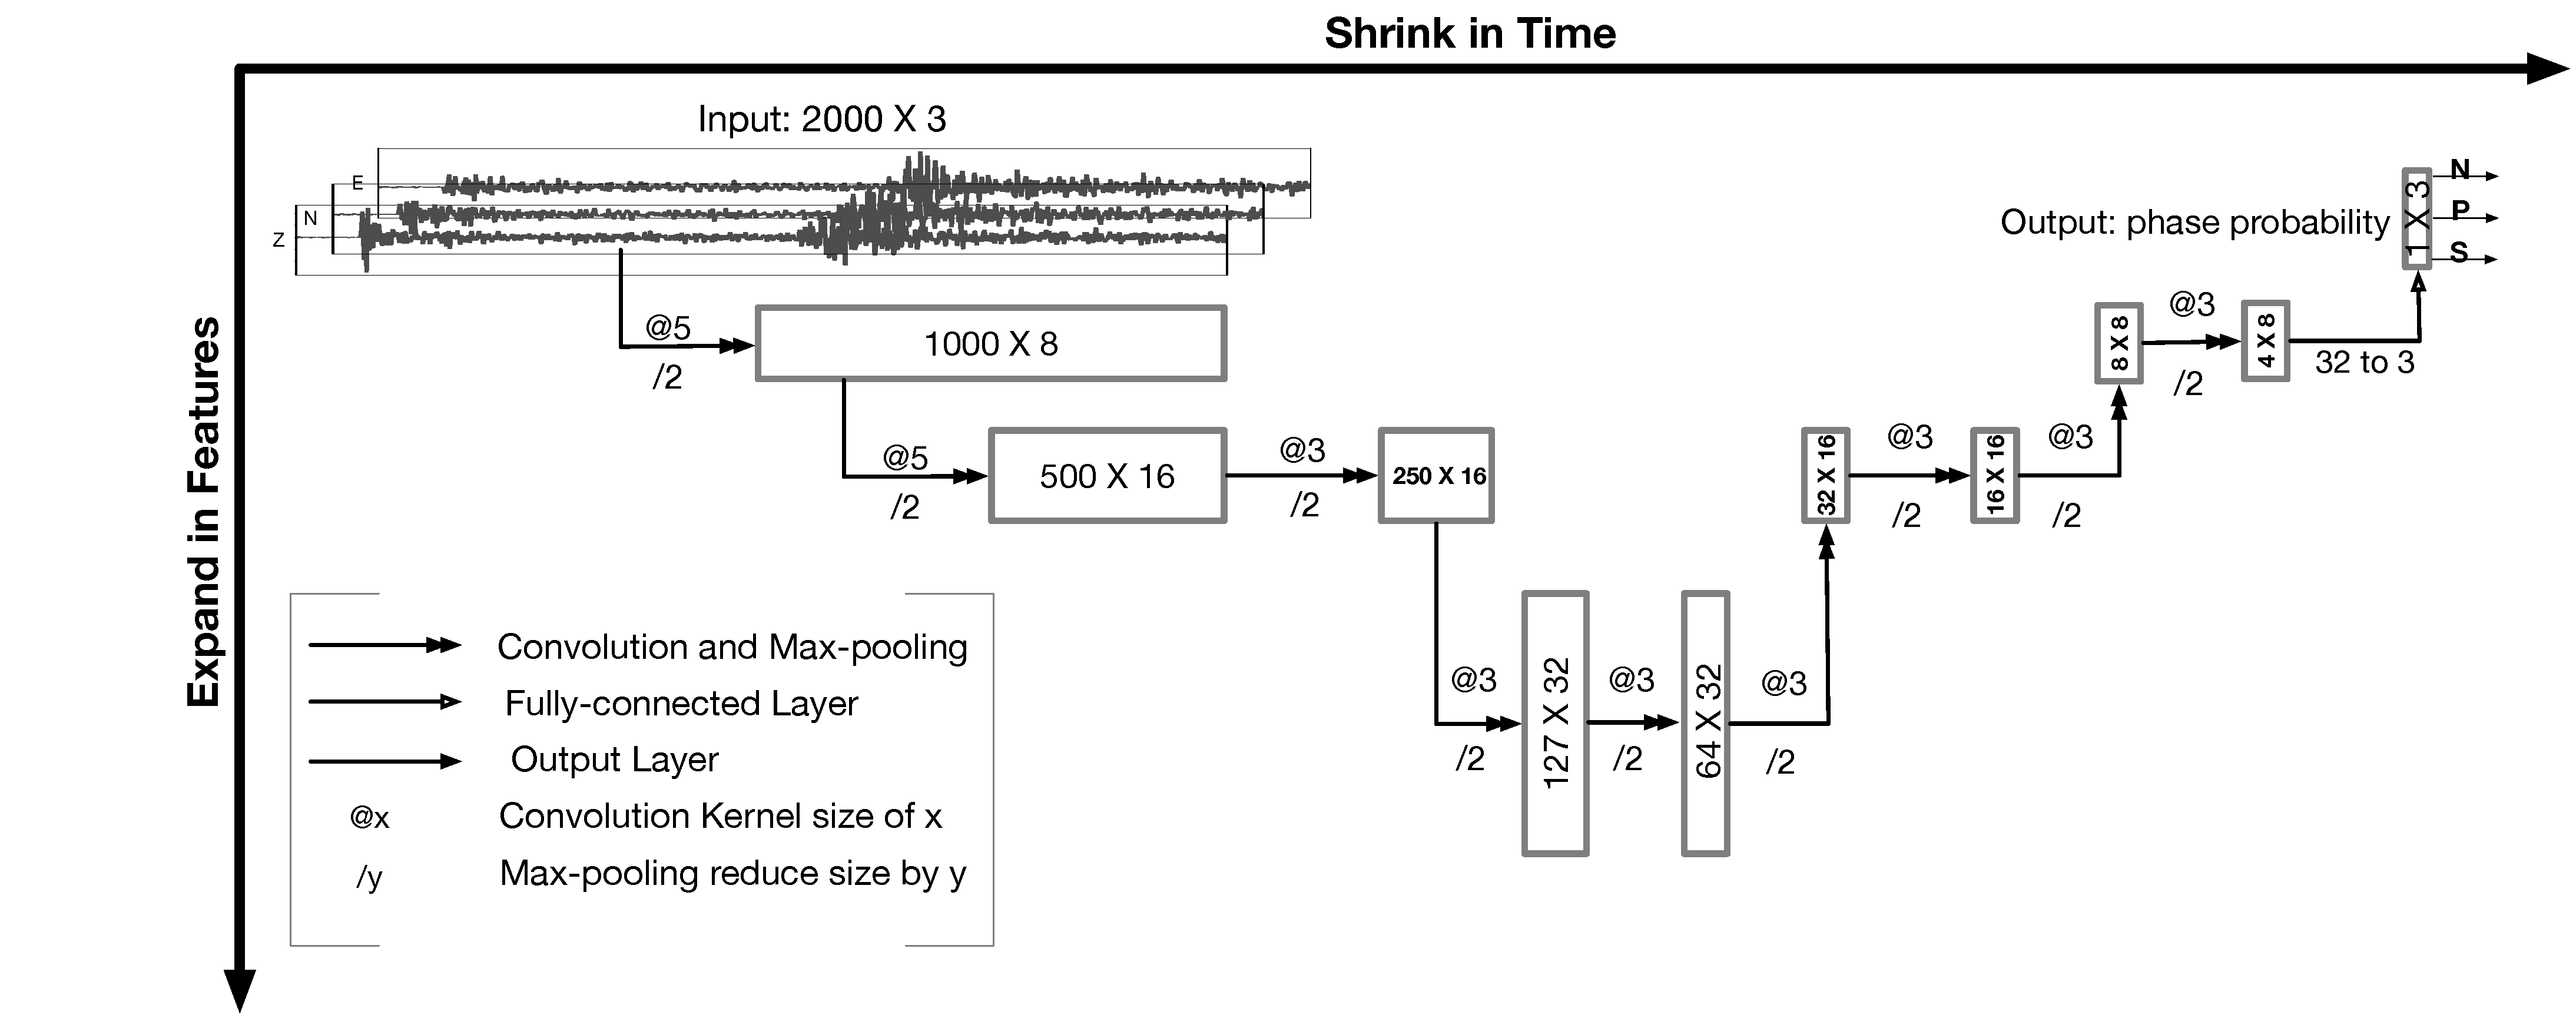
\includegraphics[width=\linewidth]{cpicv2_diagram}
    \caption{A diagram showing the data sizes in the simplified CNN network structure. Each input is a 3-C seismogram (20-s window) which shrinks in time but expands in the feature dimension as it passes through nine convolutional layers for feature extraction. The final layer is fully connected with three outputs that give the probabilities of a window being noise, P, and S phases.}
    \label{fig:cpicv2}
\end{figure}
%

The training process of the simplified \gls{cpic} model is shown in Figure~\ref{fig:train_cpicv2}.
Comparing to the training process of the original \gls{cpic} model in Section~\ref{sec:train_val}, the simplified model reaches nearly the same classification accuracy at 97.2\% vs.\ 97.4\% for the original model.
However, the training process takes more epochs to converge, and the validation accuracy in the early epochs becomes quite volatile.
The simplified model converges near the final stopping accuracy after more than 70 epochs, while the same happens for the original \gls{cpic} model within 40 epochs.
The orange curves for training in Figure~\ref{fig:train_cpicv2} resemble those in Figure~\ref{fig:train_cpicv2}, indicating a stable training process.
However, the blue curves in Figure~\ref{fig:train_cpicv2} oscillate more dramatically in Figure~\ref{fig:train_cpicv2} than those in Figure~\ref{fig:evaluate_train}.
The simplified model has less redundancy and can be more sensitive to perturbations in the input data when its weights have not gotten close to the optimal region.
Notice that there is no over-fitting observed, as expected, on the simplified model given a training set of the same size.
%
\begin{figure}
    \centering
    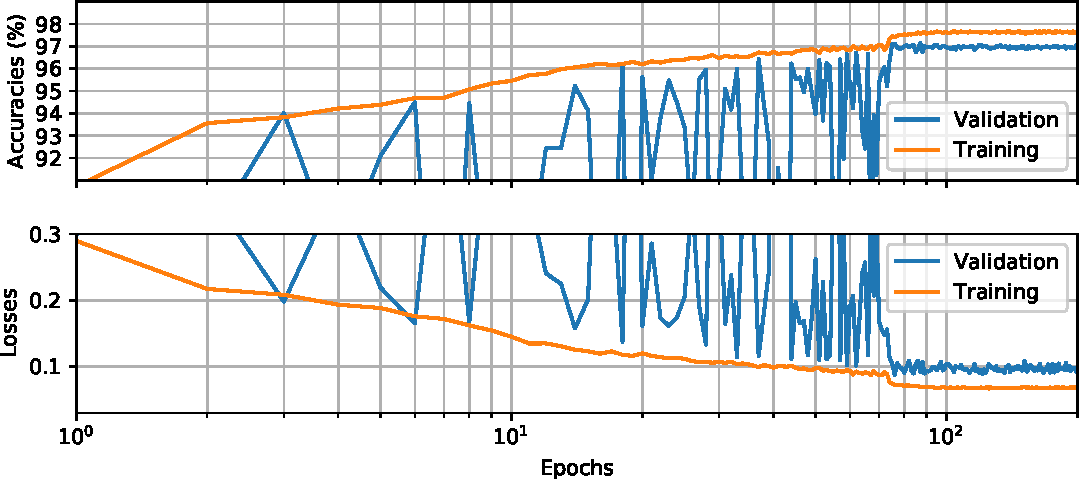
\includegraphics[width=\linewidth]{evaluate_train_cpicv2}
    \caption{Training performance of simplified \glstext{cpic} model on Wenchuan dataset: (a) classifier accuracy and (b) loss function against number of epochs for training and validation datasets during the CNN training process.}
    \label{fig:train_cpicv2}
\end{figure}
%

\section{Quantization of CNN Model}
\label{sec:quantization}
%
As demonstrated in Section~\ref{sec:weight_distribution}, the effective dynamic range of the weights in each layer of the \gls{cpic} model is relatively small.
Furthermore, the seismic waveforms recorded on a seismometer are usually represented in a fixed-point (integer) format using a wordlength between 12 and 24 bits.
It is natural to think about quantization of the \gls{cnn} model as lowering the precision of arithmetic operations, as well as reducing both the amount of computation and the memory size.
Instead of using either fixed-point or floating-point numbers, a dynamic fixed-point number has been proposed specifically for quantization in neural networks \autocite{courbariaux2014training}.
Arithmetic operations are conducted in fixed-point while keeping a separate scaling factor for each neural network layer as a floating-point number.
A specialized simulation scheme, which can be run on floating-point only \glspl{gpu}, is designed to validate the classification accuracy of the quantized \gls{cpic} model in dynamic fixed-point numbers.
Then a fine-tuning process can be used to improve the classification accuracy when the \gls{cpic} model is quantized using fewer number of bits.


\subsection{Finite Word Length Scheme}
\label{sec:finite_word_length}
%
Summarized in \textcite{gevers1993finite}, the performance degradations due to finite-precision arithmetic in the filter implementation and computations are:
%
\begin{enumerate}
    \item  quantization of the input signals into a set of discrete levels and the ensuing quantization errors
    \item overflow of the computations, which occurs when the computation results are out of the range of the fixed-point hardware capacity;
    \item accumulation of roundoff errors that occur at arithmetic operations;
    \item quantization of the filter coefficients into a  finite number of bits and the ensuing quantization errors.
\end{enumerate}
%
The first effect, input signal quantization error, depends on the \gls{adc} used on the seismic recording device.
ADC errors are usually modeled as an additive uniformly distributed white noise, which has nothing to do with the filter structure or its parameters (filter coefficients).
The other three effects are influenced by the particular implementation chosen for the filter.
The overflow effect is based on the wordlength capacity of the computing system, which occurs when the dynamic range of the signals exceeds the maximum value that can be represent with a given wordlength.
A proper scaling of the signals, which is a function of the signal dynamic range, is necessary to avoid serious errors caused by overflows.

The accumulation of roundoff errors after arithmetic operations and the errors induced by finite wordlength encoding of the filter weights are usually called \gls{fwl} effects.
As soon as an ideal model (with full precision) is implemented in a \gls{fwl} machine (an embedded device), some performance degradation due to \gls{fwl} errors is inevitable.
There are two basic ways of representing real numbers: fixed-point representation and floating-point representation.
Internally, most computing system uses a binary number system.
In \textit{fixed-point binary representation}, the ``two's complement'' number representation is the most frequently used format for signed numbers.
A real number $x$ is represented in a quantized form as
%
\begin{equation}
Q[x] = K \left( -x_0 + \sum_{i=1}^B x_i 2^{-i} \right)
\label{eq:twos}
\end{equation}
%
where $K$ is  an arbitrary scale factor and the $x_i$ are binary digits which are either 0 or 1.
Note that the first bit, $x_0$, controls the sign of $x$ and is also known as the \textit{sign bit}.
If $x_0 = 0$, $0 \leq x \leq K$ is nonnegative; if $x_0 =1$, $-K \leq x < 0$ is negative.
The number inside the parentheses of \eqref{eq:twos} is between $-1$ and $+1$.
Thus, any number with magnitude less than $K$ can be uniquely represented by \eqref{eq:twos}.
When $B$ is infinity, the representation is perfect; otherwise, when $B$ is finite, we encounter a \gls{fwl} effect.

The quantized representation is in the range of $-K \leq Q[x] \leq K -q$, where $q$ is the smallest difference between any two of the total $2^{B+1}$ numbers, known as the  \textit{quantization step size}.
Notice that the quantization error $|x - Q(x)| \leq q$ for any $x$, and is uniformly distributed between $- q/2$ and $+q/2$ along the $x$-axis regardless of the magnitude of $x$.
%% TODO: rounding
%%
%\begin{figure}
%    \centering
%    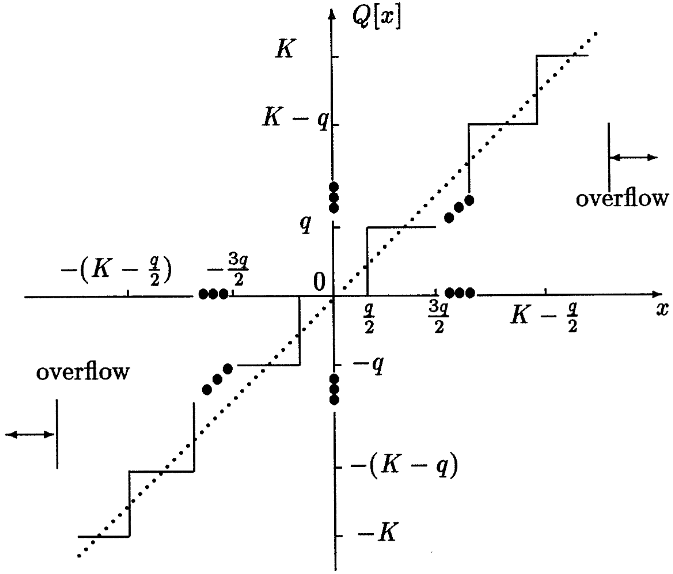
\includegraphics[width=0.9\linewidth]{quantization_scheme}
%    \caption{Demonstration of two's complement quantization scheme in Figure 2.3 of \textcite{gevers1993finite}.}
%\end{figure}
%
%The \textit{floating-point binary representation} of a number $x$ is
%%
%\begin{equation}
%F[x] = x_m 2 ^ x_e
%\label{eq:floating}
%\end{equation}
%%
%where $x_m$ is called the \textit{mantissa}, and $x_e$ is called the \textit{exponent}.
%It is not hard to see that the resolution between two successive floating-point numbers depends on their magnitudes.
%Thus, the quantization error is proportional the magnitude, i.e. $|x - Q[x]| = \epsilon |x|$.
With proper choice of the scaling factor $K$ in \eqref{eq:twos}, the dynamic range of $Q[x]$ can be made identical to that of a floating-point number with the same number of bits.
A fundamental difference is that the quantization error of fixed-point numbers is identical all through the dynamic range, while that of floating-point numbers is small for small numbers and large for large numbers.
When the relative error is more relevant than the absolute one, which is often the case, floating-point representations typically deliver a better range\,--\,precision tradeoff than fixed-point ones.
However, arithmetic operations with floating-point numbers are more complicated, so floating-point coprocessors are often added in modern day computers when computation speed is an essential factor.

The dataflow in the  \gls{fc} and the \gls{conv}s consists many \gls{mac} operations as demonstrated by Figure~\ref{fig:fixed_point_arithmetic}.  
The feature maps are multiplied with the filter weights, and their results are accumulated to form the outputs.
For example, a feature map of $m$ bits and filter weights of $n$ bits are multiplied and accumulated using an adder tree such as in Figure~\ref{fig:fixed_point_arithmetic}.  
The multiplication results in an $m + n$ bit output product, and the additions at each level of the tree add one more bit.
In the last level, the bit-width is $m+n+ \log_2(c)$, where $c$ is the number of multiplications per output channel.  
After filtering, a bias is added to form the output which is then truncated to the lower precision representation by the shifters.
Thus, our goal in quantization design is to find a good balance between reducing the bit-widths ($m$ and $n$) and maintaining a good classification accuracy for the \gls{cnn}.
For simplicity, $m$ and $n$ are chosen to be the same in this study.
%
\begin{figure}
    \centering
    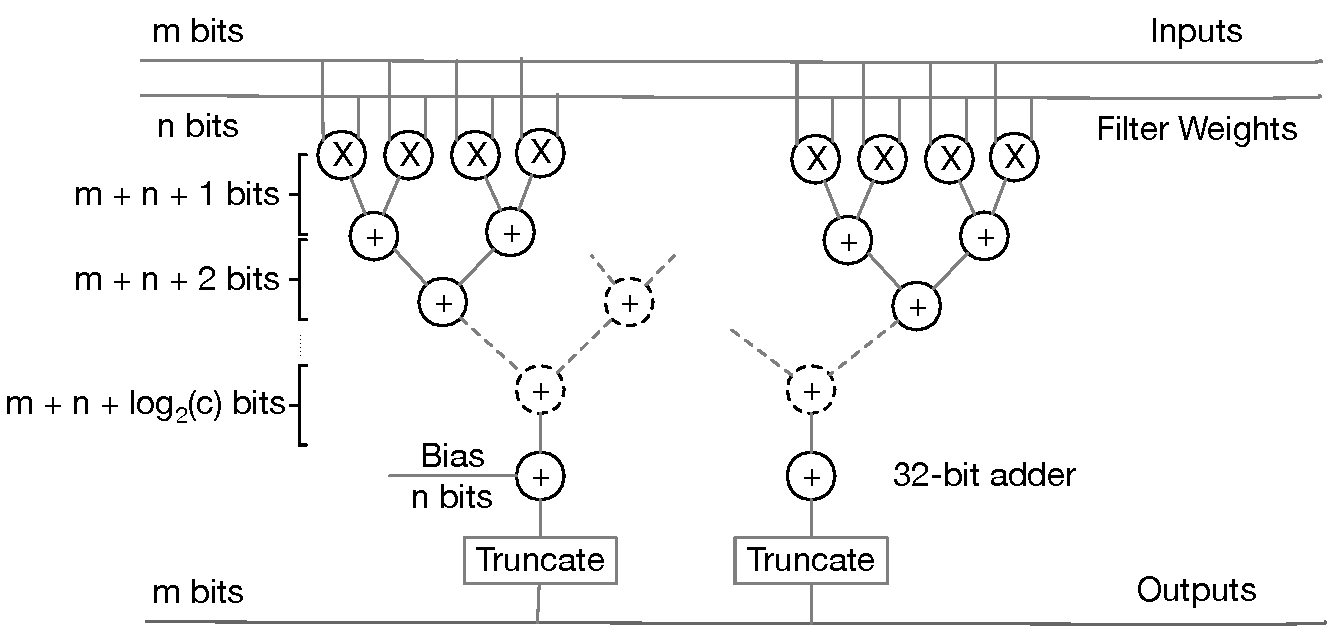
\includegraphics[width=\columnwidth]{fixed_point_arithmetic}
    \caption{Fixed-point number operation in convolutional neural networks. Adapted from Figure 5.1 in \textcite{gysel2016ristretto}.}
    \label{fig:fixed_point_arithmetic}
\end{figure}
%

\subsection{Inference using the Quantized CNN Model}
\label{sec:inference}
%
To accommodate the large dynamic range difference in each layer of the neural network, a \textit{dynamic fixed-point} scheme was proposed for neural networks \autocite{courbariaux2014training}.
It was proposed originally for faster training; however, \textcite{gysel2016hardware} later demonstrated that this dynamic fixed-point scheme has more value in approximating \gls{nn} models during inference.

Similar to a block floating-point number format, the dynamic fixed-point representation uses a scaling factor $S^l$, which is a power of $2$, represented in floating-point for scaling each \gls{nn} layer.
Effectively, $S^l$ determines the location of the binary point of each number in that layer and thus controls the the fractional length of the fixed-point number.
The filter weights are still represented as fixed-point numbers using this shared scaling factor as in \eqref{eq:dynamic}:
%
\begin{equation}
x^l = S^l \left( -x_0^l + \sum_{i=1}^B 2^{-i} \right)
\label{eq:dynamic}
\end{equation}
%
Comparing with \eqref{eq:twos}, each layer has a dynamically changing scale factor $S^l$ instead of a global fixed scaling factor $K$.
However, the same $S^l$ is shared within a single \gls{nn} layer, which is different from the exponent $x_e$ in floating-point which can vary from weight to weight.
More importantly, the evaluation of this shared scaling factor can be delayed until the last layer of each branch.
Since the \gls{cpic} model only has one branch, there will be only one global scaling factor in floating-point at the end.
During \gls{cnn} inference, the filter outputs are computed in fixed-point, where only the relative values, instead of the absolute values are tracked.
Since both \gls{relu} and max-pooling, at the layer output, operate based on comparing numbers, relative values are sufficient.

%
\begin{figure}
    \centering
    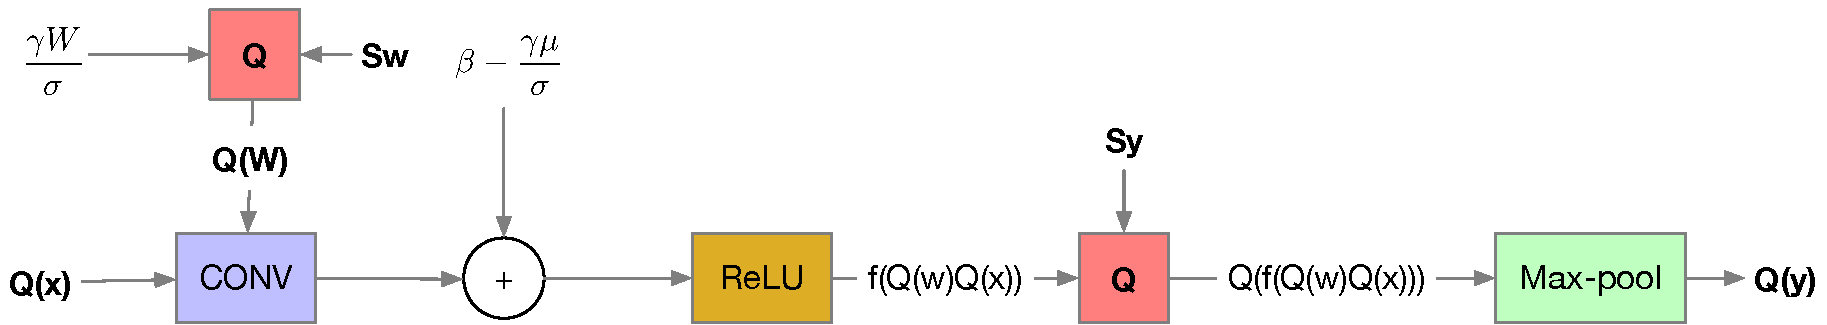
\includegraphics[width=\linewidth]{quant_inference}
    \caption{Flow diagram of a \glstext{conv} quantized using the dynamic fixed-point number system. Notice that the batch norm has been absorbed into the filter weights $W$. There are two scaling factors: $S_w$ for filter weights and $S_y$ for feature maps.}
    \label{fig:quant_inference}
\end{figure}
%
Figure~\ref{fig:quant_inference} shows the overall inference pipeline of the quantized \gls{cnn} model.
The input $x$ and filter weights $W$ are both quantized into a $B$-bit representation as $Q(x)$ and $Q(W)$ respectively.
The \gls{conv} output will be a $4B$-bit fixed-point representation $Q(W)Q(x)$, which will be bottom clipped by \gls{relu}.
The precision of the nonlinearly activated data $f(Q(W)Q(x))$ will then be reduced to $B$ bits before passing into the max-pooling layer.
Notice that the $Q$ block can be performed after the max-pooling layer; however, it is faster to find the max value in the fixed-point representation rather than in floating-point.
There are two scaling factors, $S_w$ and $S_y$, involved in the process.
Combining those with the scaling factors $S'_w$ and $S'_y$ from the previous layer, denoted as $S_x = S'_w S'_y$, the global scaling factor can be computed as
%
\begin{equation}
S = S_0 \prod_{i=1}^{N} S_w^i S_y^i
\label{eq:global_scale}
\end{equation}
%
where $S_0$ is the input scaling factor, $S_w^i$ and $S_y^i$ are the dynamic scaling factors for the $i^\text{th}$ layer, and $N$ is the number of layers.

The batch norm layers are omitted in Figure~\ref{fig:quant_inference} since they are usually absorbed into the previous \gls{conv}.
Indeed, the \gls{conv} operation
%
\begin{equation}
y = Wx + b
\label{eq:conv}
\end{equation}
%
where $W$ is the filter weights and $b$ is the filter bias, can be combined with
the \gls{bn} operation to obtain
\begin{equation}
y = \gamma \left(\frac{x - \mu}{\sigma}\right) + \beta
\label{eq:bn}
\end{equation}
%
where $\mu$ is the sample mean, $\sigma$ is the sample standard deviation in the current batch (a collection of training samples), $\gamma$ is the scaling factor and $\beta$ is the bias factor, both of which are learnable parameters in the training process.
The result of combining \eqref{eq:conv} and \eqref{eq:bn} into a \gls{conv} operation is \eqref{eq:absorb} below
\begin{equation}
     y = \gamma \left(\frac{Wx + b - \mu}{\sigma}\right) + \beta = W' x + b'
     \label{eq:absorb}
\end{equation}
where $W' = \frac{\gamma W}{\sigma}$ and $b' = \beta - \frac{\gamma \mu}{\sigma}$ are the filter weights and bias of the new \gls{conv} with the \gls{bn} absorbed.
This is also the reason that \glspl{conv} followed by a \gls{bn} do not need a bias in the filter coefficients.%
On the other hand, the \gls{bn} dynamically estimate the sample mean and variance of each batch during the training process while using fixed values during validation.
The dynamically estimated batch statistics are accumulated by an exponential moving average, i.e.,
%
\begin{equation}
S_t = \left\{
\begin{aligned}
&Y_1, & t= 1\\
&\alpha Y_t + (1 - \alpha) S_{t-1}, & t > 1
\end{aligned}
\right.
\end{equation}
%
where $Y_t$ is the estimator of the current batch, $S_t$ is the accumulated estimator of all batches, and $\alpha$ is the exponential decay of the weighting.

Given enough number of bits, the direct quantization of most \gls{cnn} models is sufficient to approximate the original floating-point model as observed in \textcite{krishnamoorthi2018quantizing}.
However, a fine-tuning process can be developed to obtain improvements over the directly quantized models.

\subsection{Fine-tuning the Quantized CNN Model}
\label{sec:fine_tuning}
%
Fine-tuning of a quantized \gls{cpic} model is based on a simple assumption.
The optimal quantized model should be similar enough to the original floating-point model that with small tweaking of filter weights, the overall classification accuracy can be recovered.
Gradient-based approaches can still be used to fine-tune the quantized weights of the neural network; however, an approximation of the derivative of the quantizer operator is needed for the chain rule to pass the gradient during the backpropagation process.
The quantizer is a nonlinear and non-differentiable function as shown in Figure~\ref{fig:quant_derivative} (left), but the piecewise linear approximation in 
Figure~\ref{fig:quant_derivative} (right) is a function commonly used as a proxy for the quantizer's derivative.
The exact outputs of the nonlinear quantizer are used in the forward pass, while the approximated derivatives are used in the backward pass.
This discrepancy between forward and backward passes should be negligible if the quantizer has enough number of bits.
Indeed, as the number of bits in the quantizer increases, the step size decreases and the closer two functions in Figure~\ref{fig:quant_derivative} resemble each other.
When an infinite number of bits are available, these two functions are equivalent.
%
\begin{figure}
    \centering
    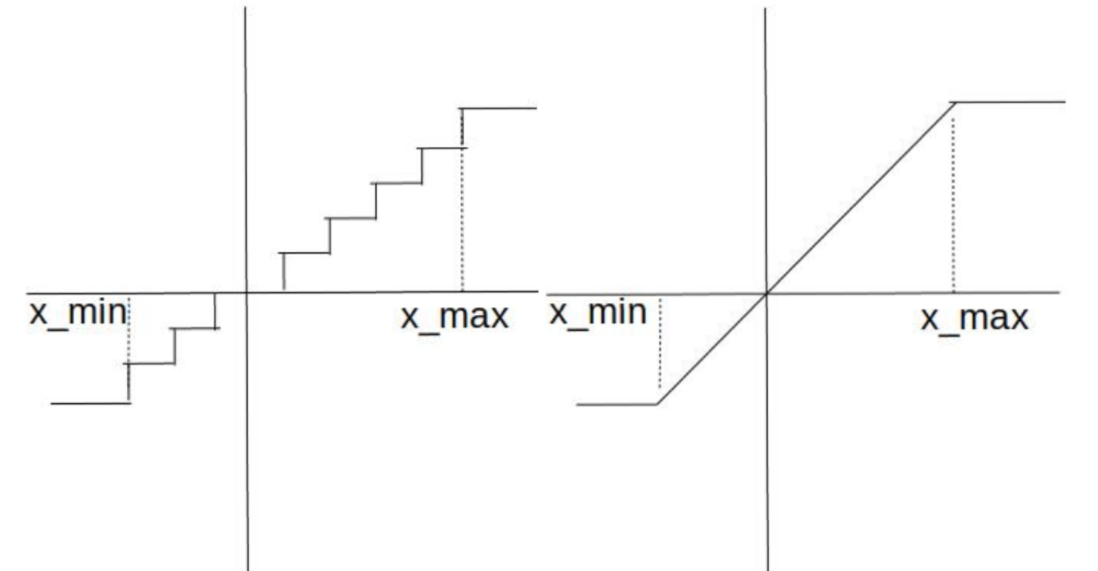
\includegraphics[width=0.68\linewidth]{quant_derivative}
    \caption{Simulated quantizer (left) and an approximation (right) for the purpose of calculating its derivative, from Figure 1 in \textcite{krishnamoorthi2018quantizing}.}
    \label{fig:quant_derivative}
\end{figure}
%

Different input data will result in a different scaling factor $S_y^i$ for the $i^\text{th}$ layer; however, when deploying the model, each layer needs to have a fixed scaling factor.
One could look at all the known input data and use the most conservative scaling factor to avoid any possible overflow problem.
However, this practice almost always results in a too conservative choice that sacrifices a significant amount of resolution for some rarely occurring extreme values.
A reasonable amount of clipping is instead allowable, but it is hard to know in advance the exact amount of clipping which can be tolerated.
In fact, these scaling factors on each layer can also be learned during the fine-tuning process.
Similar to the sample mean and sample standard deviation in the \gls{bn}, we use an exponential moving average to record the instantaneous scaling factor each time data pass through the quantized model.
Once the fine-tuning is finished, the exponential moving average has seen the entire training set multiple times with different combinations.
Each time, the exponential moving average records the most conservative choice on the current training batch with $\alpha=0.3$.
When a small portion of those training data has large magnitudes, it only affects the current batch.
In the long run, the exponential moving average will smooth the overall scaling factor estimation, allowing a few overflows on some batches while being conservative for most batches.
This behavior tries to find the optimal scaling factor that uses the dynamic range most effectively without explicitly validating all possible scaling factor choices on the entire training dataset.
Some signal saturation due to the overflow effect is acceptable here because the output activation map of the convolutional layer will be passed into another nonlinear \gls{relu} activation function. 
The existence of these nonlinearities is expected by the \gls{cnn} model. 
Thus, the degradation of performance can be partially recovered via updating the weight values during fine-tuning process.

Another challenge for fine-tuning the \gls{cpic} model, in particular, is the \gls{bn}.
Since the \gls{bn} will be absorbed into the previous \gls{conv}, the quantization of the combined \gls{conv} needs to be simulated during the training process.
Both $\mu$ and $\sigma$ need to be estimated for each training batch, so the \gls{conv} needs to be run twice on each iteration.
As shown in Figure~\ref{fig:quant_training_bn}, during the training process, feature maps are passed into the \gls{conv} with full precision weights followed by the \gls{bn}.
This is used to estimate the sample mean $\mu$ and sample standard deviation $\sigma$ as accurately as possible.
The estimated $\mu$ and $\sigma$ are then used to simulate the \gls{bn} value for absorption.
The new \gls{conv} with the \gls{bn} absorbed is then quantized following the same procedure shown in Figure~\ref{fig:quant_inference}.
During inference, the new bias $b'$ is added back after the \gls{conv} whose weights include the absorbed \gls{bn} coefficients as shown in Figure~\ref{fig:quant_inference_bn}.
%
\begin{figure}
    \centering
    %
    \begin{subfigure}{\linewidth}
        \centering
        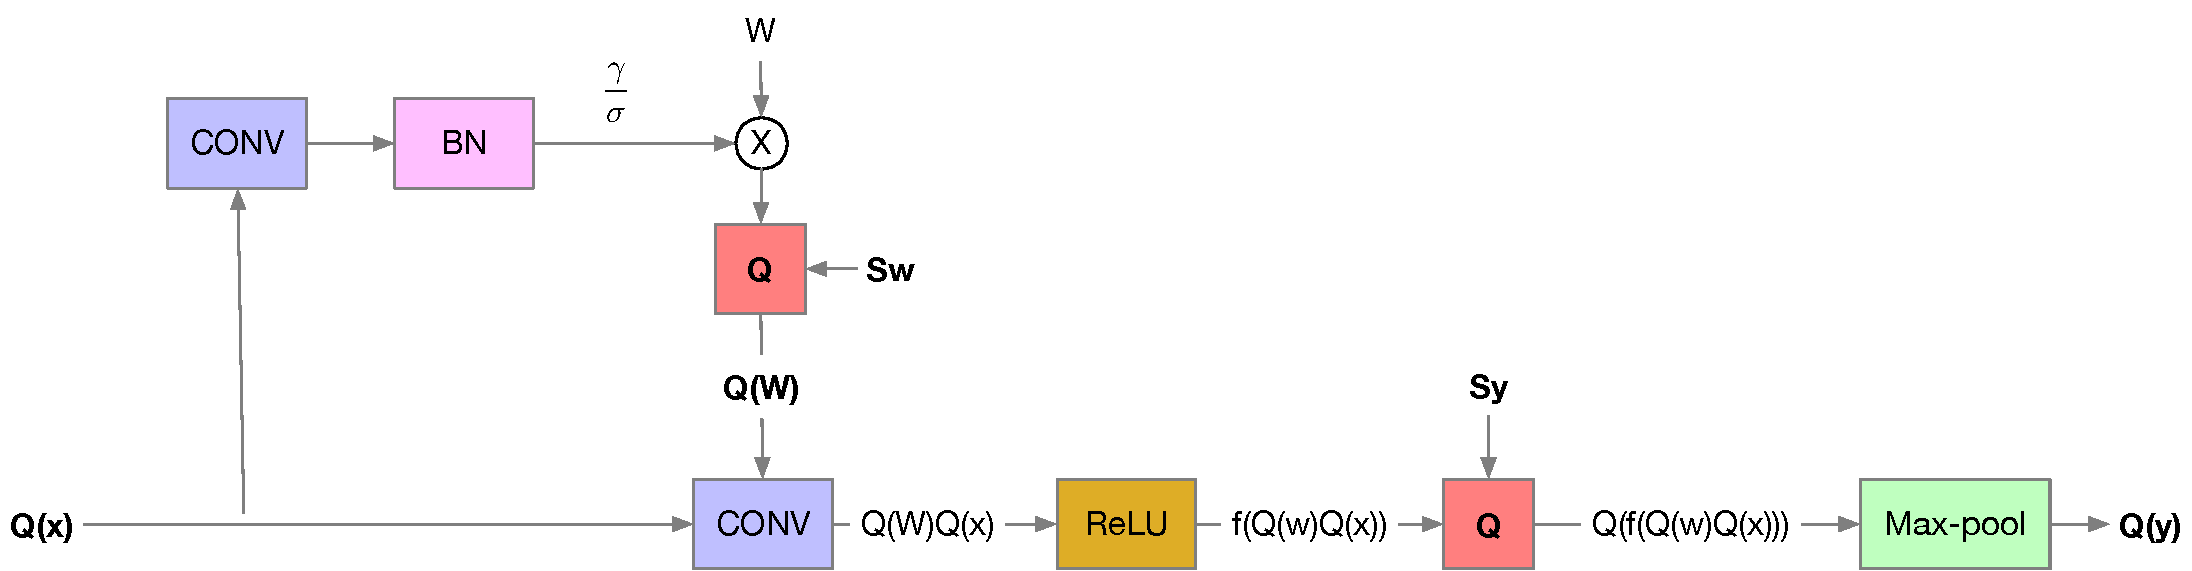
\includegraphics[width=\linewidth]{quant_train_bn}
        \caption{Training}
        \label{fig:quant_training_bn}
    \end{subfigure}
    %
    %
    \begin{subfigure}{\linewidth}
        \centering
        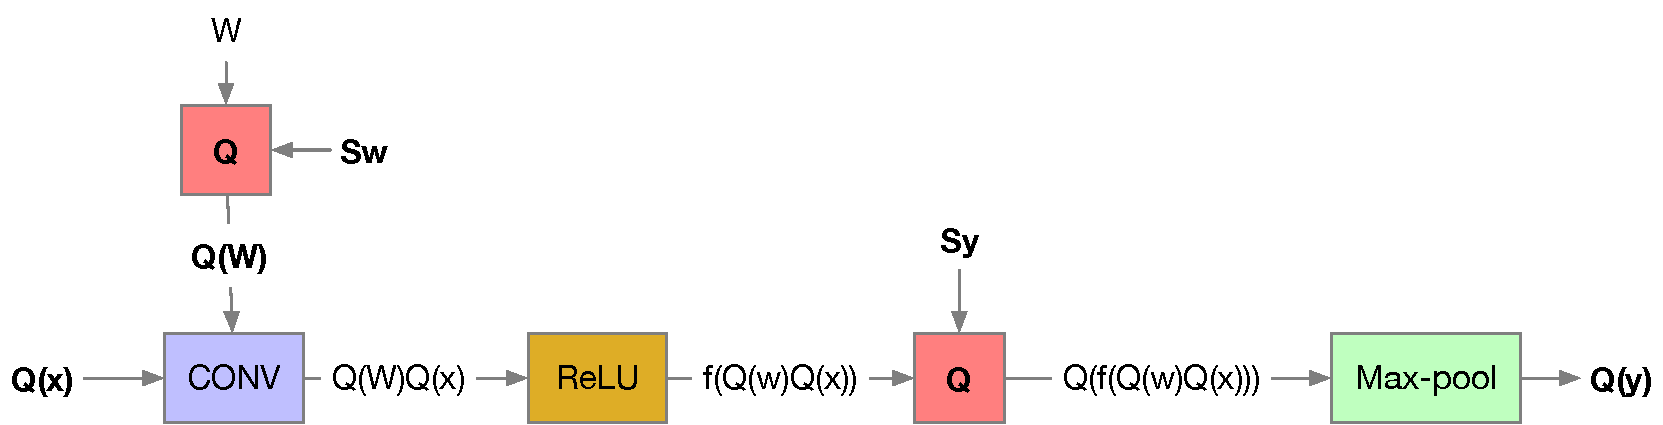
\includegraphics[width=\linewidth]{quant_inference_bn}
        \caption{Inference}
        \label{fig:quant_inference_bn}
    \end{subfigure}
    %
    \caption{Fine-tuning process for quantized \glstext{cnn} model with the \glstext{bn} incorporated into the \glstext{conv}.}
    \label{fig:quant_bn}
\end{figure}

Using the training and inference scheme shown in Figure~\ref{fig:quant_bn}, the simplified \gls{cpic} from Section~\ref{sec:simplified_model} is quantized into lower precision.
Figure~\ref{fig:train_cpicv2_8bit} shows the evolution of the training and validation processes vs.\ epochs for the quantized model in 8-bit fixed-point.
After an initial drop in validation accuracy, the fine-tuning process gradually recovers most of this loss of classification accuracy due to quantization in about 70 epochs.
So, the fine-tuning processing was run for 100 epochs instead 200.

Table~\ref{tab:quant} summarizes results for different numbers of bits: the simplified floating-point model is quantized into dynamic fixed-point numbers using 12, 10, 8, 6, and 4 bits.
The most recent high-end seismic sensors record waveforms with 24-bit ADCs, while most inexpensive devices record with at least 12 bits. 
[TODO] say what we stopped at 12 bit.
The first row of Table~\ref{tab:quant} shows the classification accuracy difference between the simplified \gls{cpic} model in floating-point and the lower-precision model with only the filter weights quantized.
This is a reference point for other quantization experiments.
If the assumption that the quantized model is similar to the floating-point case holds, the fine-tuned model should never have classification accuracy higher than the ones shown in the first row.
This is true for all but the 4-bit case where the fine-tuned model performs significantly better than the weight-only quantized model.
In this case, the weights in the fine-tuned model must be dramatically different from the original floating-point numbers making it inappropriate to use the proposed scheme to fine-tune the model for classification recovery.
Indeed, the step-function-shaped 4-bit quantizer is significantly different from a 45-degree line making the approximation shown in Figure~\ref{fig:quant_derivative} invalid.
Notice that the classification accuracy is better without fine-tuning in the case of 12 bits.
This agrees with our assumption that the optimal quantized model is close to the floating-point model given enough number precision.
%
\begin{figure}
    \centering
    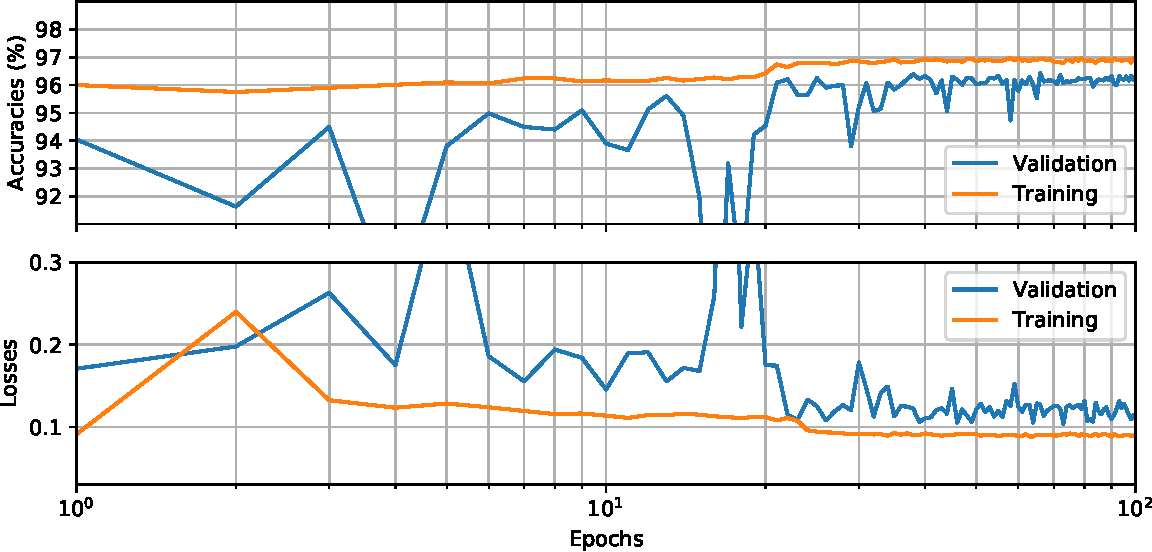
\includegraphics[width=\linewidth]{evaluate_train_quant_8bit}
    \caption{Training performance of simplified \glstext{cpic} model quantized with 8-bit fixed-point numbers on Wenchuan dataset: (a) classifier accuracy and (b) loss function against number of epochs for training and validation datasets during the CNN training process.}
    \label{fig:train_cpicv2_8bit}
\end{figure}
%
%
\begin{table}
    \centering
    \caption{Validation accuracy of the quantized \glstext{cpic} fixed-point model 
%    	compared and the simplified floating-point model (97.2\%) on Wenchuan dataset
 with a varying number of bits. Cases with less than $1\%$ accuracy differences are marked in green; those with differences between $1\%$ and $5\%$ in orange; those with differences over $5\%$  in red. The first row is unrealistic where filter weights are quantized but the feature maps are not, but it serves as a reference.}
    \label{tab:quant}
%    \begin{tabular}{l c c c c c }
%        \toprule
%        Number of Bits & 12 & 10 & 8 & 6 & 4\\
%        \midrule
%        Weight-only quantization (\%) & \colorbox{white}{0.01} & \colorbox{white}{-0.05} & \colorbox{white}{-0.13} & \colorbox{orange}{-1.24}  & \colorbox{red}{-23.67}\\
%        Fully quantized model (\%) & \colorbox{green}{-0.03} & \colorbox{green}{-0.42} & \colorbox{orange}{-1.96} & \colorbox{red}{-19.28}  & \colorbox{red}{-40.93} \\
%        Fine-tuned one epoch (\%) & \colorbox{green}{-0.26} & \colorbox{green}{-0.45} & \colorbox{orange}{-2.55} & \colorbox{red}{-7.75} & \colorbox{red}{-27.32}\\
%        Fine-tuned 100 epochs (\%) & \colorbox{green}{-0.08} & \colorbox{green}{-0.20} & \colorbox{green}{-0.70} & \colorbox{orange}{-4.51} & \colorbox{red}{-11.55}\\
%        \bottomrule
%    \end{tabular}
%    %
    \begin{tabular}{l c c c c c }
        \toprule
        Number of Bits & 12 & 10 & 8 & 6 & 4\\
        \midrule
        Weight-only quantization (\%) & \colorbox{white}{97.22} & \colorbox{white}{97.16} & \colorbox{white}{97.08} & \colorbox{orange}{95.97}  & \colorbox{red}{73.54}\\
        Fully quantized model (\%) & \colorbox{green}{97.18} & \colorbox{green}{96.79} & \colorbox{orange}{95.25} & \colorbox{red}{77.93}  & \colorbox{red}{56.82} \\
        Fine-tuned one epoch (\%) & \colorbox{green}{96.95} & \colorbox{green}{96.76} & \colorbox{orange}{94.66} & \colorbox{red}{89.46} & \colorbox{red}{69.89}\\
        Fine-tuned 100 epochs (\%) & \colorbox{green}{97.13} & \colorbox{green}{97.01} & \colorbox{green}{96.51} & \colorbox{orange}{92.70} & \colorbox{red}{85.66}\\
        \bottomrule
    \end{tabular}
\end{table}
%

The fully quantized models are shown in the second row of Table~\ref{tab:quant}.
The value is slightly inflated as the exponential moving average for scaling factor estimation has been turned off for these models.
The scaling factors used in validating them are dynamically computed to avoid any possible overflow problem.
Since it is impossible to have a different scaling factor for different input data, the accuracy shown on the second line is slightly better than it should be.
After one epoch of training, the exponential moving averages for the scaling factors have seen all training data; so the averages of the scaling factors does not change much for the model on the third row of Table~\ref{tab:quant}.
Notice that the fine-tuning process completely recovers the classification accuracy for a 12-bit model.
The 10-bit and 8-bit cases can be recovered with less than 1\% difference in classification accuracy.
However, the 6-bit model can only be recovered within a 5\% difference making it borderline for feasible usage.
The 4-bit model, as discussed before, is not appropriate for the proposed fine-tuning process and has more than a 10\% drop in classification accuracy even after the fine-tuning process.

Currently, the quantization process is simulated on \glspl{gpu} in floating-point with artificially reduced precision.
Thus it can correctly model the noise and classification error due to reduced precision; however, the simulated fine-tuning process for the quantized model is much slower than its counterpart for a floating-point model.
As more and more general purpose \glspl{gpu} start to support half-precision, or even quarter-precision integers, this fine-tuning may be conducted with actual fixed-point numbers, which would significantly improve its speed.
Moreover, when the embedded processors start to support the acceleration of matrix-matrix multiplication of low-precision integers, we may even be able to fine-tune the \gls{cpic} model directly on the embedded processor of an edge device.

\section{Deployment on Embedded Devices}
\label{sec:rbp}
%
The simplified \gls{cpic} model quantized in dynamic fixed-point is now ready for deployment on embedded devices.
Due to the lack of compatible firmware on the Raspberry Pi board, the evaluation of this deployment of quantized models must be deferred to future work.
Note that this thesis provides all the necessary tools for converting a validated floating-point model to the target fixed-point model.
In the this section, the floating-point number models are benchmarked instead.

The original \gls{cpic} model and simplified \gls{cpic} models from Section~\ref{sec:simplification} are tested on a four-minute segment of 3-C waveforms from the Mariana dataset.
As shown in Figure~\ref{fig:rbp}, both P and S-wave characteristic functions from the two  models have a peak near the corresponding manual pick times.
Although it is counterintuitive, arrivals of \glspl{pwave} are more challenging to pick on the Mariana dataset than those of \glspl{swave}.
This is primarily due to the source mechanism in the Mariana subduction zone which produces \gls{pwave} arrivals with gradually increasing magnitude instead of more abrupt changes from the noise floor. 
This is very different from cases in the Wenchuan dataset that the \gls{cpic} model was originally trained on.
Thus, having the \gls{cpic} model fine-tuned on a small subset of the Mariana dataset should help with the picking results.
Indeed, when fine-tuned on 2,000 samples from the Mariana dataset, the simplified \gls{cpic} model shows a significant improvement in picking accuracy for \glspl{pwave} as shown in Figure~\ref{fig:rbp}(f).
However, this is not true for the original \gls{cpic} model.
When fine-tuned on 2,000 samples, the picking results hardly change for any of the predicted \gls{pwave} arrival times in Figure~\ref{fig:rbp}(c).
We do observe some improvement in denying surface waves that come after \glspl{swave}, which were mistakenly recognized as \glspl{swave} previously without fine-tuning.
After expanding the number of samples for fine-tuning to 14,000, the picking results in Figure~\ref{fig:rbp}(d) show some improvement for \glspl{pwave}.
This phenomenon may be caused by the difference in the model sizes.
The original \gls{cpic} model has more than ten times the number of parameters compared to the simplified model, which means it naturally requires more training samples to reach a stable model during the fine-tuning process. 
%
\begin{figure}
    \centering
    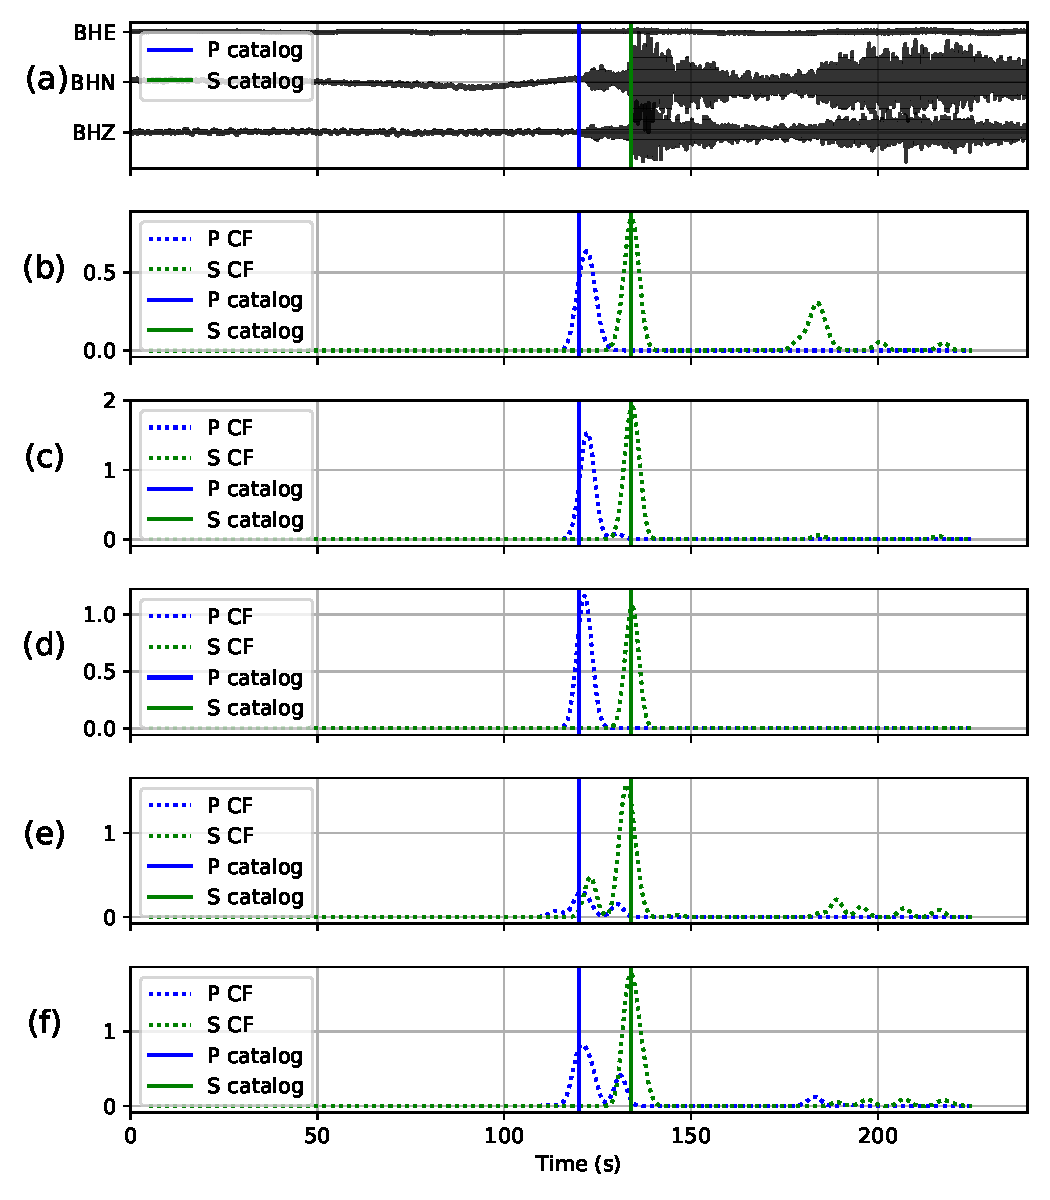
\includegraphics[width=\columnwidth]{rbp}
    \caption{Picking results for five \gls{cpic} models on a four-minute 3-C waveform from Mariana dataset. The plots from top to bottom panels are (a) three-component waveform; \gls{pwave} and \gls{swave} picking characteristic functions of (b) original \gls{cpic} model trained on Wenchuan dataset; (c) original \gls{cpic} model fine-tuned on 2,000 samples from Mariana dataset; (d) original \gls{cpic} model fine-tuned on 16,000 samples from Mariana dataset; (e) simplified \gls{cpic} model trained on Wenchuan dataset; and (f) simplified \gls{cpic} model fine-tuned on 2,000 samples from Mariana dataset. Note that the vertical blue and green lines indicate manually picked arrival times for \gls{pwave} and \gls{swave}, respectively.}
    \label{fig:rbp}
\end{figure}
%

When comparing the computation time used for processing such four-minute waveform, the simplified model is consistently faster than the original \gls{cpic} model.
Shown in Table~\ref{tab:benchmark_time}, the time consumed by simplified model is about half of that by original \gls{cpic} model for both i7 laptop and Raspberry Pi device.
This makes the simplified model more favorable.
Notice that there is no \gls{gpu} used for both testing cases.
Computation time on Raspberry Pi is roughly 100 times of that on the i7 laptop since both the CPU clock frequency and the RAM speed on the Raspberry Pi is considerable smaller than those on the i7 laptop.
However, since the computation times on both cases are significantly less than the signal duration, it is feasible to implement a real-time processing system both i7 processors as well as the Raspberry Pi devices.
%
\begin{table}
    \centering
    \caption{Benchmark of \gls{cpic} model computation times on Core i7 laptop vs.\ Raspberry Pi device processing a four-minute three-channel waveform from Mariana dataset.}
    \label{tab:benchmark_time}
    \scalebox{0.8}{
        \begin{tabular}{l c c c c}
            \toprule
            Model & Original CPIC & Fine-tuned Original CPIC & Simplified CPIC & Fine-tuned Simplified CPIC \\
            \midrule
            i7 Laptop  & 0.65\,s & 0.55\,s & 0.26\,s & 0.26\,s \\
            Raspberry Pi  & 66.47\,s & 66.68\,s & 34.09\,s & 37.68\,s \\
            \bottomrule
    \end{tabular}}
\end{table}
%

Although modern hardware accelerators for floating-point arithmetic usually claim comparable efficiency to their fixed-point counterparts, the fixed-point accelerators are still cheaper to implement, consume less power, and are more ubiquitous on low-end embedded devices.
Since seismic waveforms are originally recorded in fixed-point numbers, processing the data in fixed-point also has the advantage of avoiding continuously converting input waveforms from fixed-point numbers to floating-point numbers.
Finally, notice that many fixed-point processors have the basic processor working at 4-bit word length.
Higher precision bit computation is conducted by combining multiple basic processors.
This makes selecting the number of quantization bits favor using a multiple of four, e.g., 12-bit and 8-bit choices in Table~\ref{tab:quant} would be preferred.



\begin{singlespace}  % use single-line spacing for multi-line text within a single reference
	\setlength\bibitemsep{\baselineskip}  %manually set separation between items in bibliography to double space
	\printbibliography[title={References}]
\end{singlespace}

\end{document}
